% \documentclass[bachelor]{seuthesis} % 本科
\documentclass[master]{seuthesis} % 硕士
% \documentclass[doctor]{seuthesis} % 博士
% \documentclass[engineering]{seuthesis} % 工程硕士

% 这里是导言区
\usepackage{etoolbox}
\usepackage{algorithm}
\usepackage{algorithmic}
\begin{document}
%%%%%%%%%%%%%%%%%%%%%%%%以下内容先一键注释掉,等到成文之后再加入编译%%%%%%%%%%%%%%%%%%%%%%%%%%%
%\categorynumber{TN92} % 分类采用《中国图书资料分类法》
%\UDC{621.3}            %《国际十进分类法UDC》 的类号
%\secretlevel{公开}    %学位论文密级分为"公开"、"内部"、"秘密"和"机密"四种
%\studentid{130657}   %学号要完整,前面的零不能省略。
%\title{可见光多波段通信系统自适应传输\ \ 技术研究}{}{Research On Adaptive Transmission Technology Of Multi Visible Light Communication System}{}
%\author{吴满}{Man Wu}
%%\author{}{~}
%\advisor{赵春明}{教授}{Chunming Zhao}{Prof.}
%%\advisor{}{}{~}{~}
%%\coadvisor{张\quad{}华}{副教授}{Hua Zhang}{Associate Prof.}  % 没有可以不填
%
%\degree{工学硕士} % 详细学位名称
%\major{信息与通信工程}
%\submajor{通信与信息系统}
%\defenddate{2016年1月24日}
%%\defenddate{}
%%\authorizedate{2015年3月20日}
%\authorizedate{}
%\department{信息科学与工程学院}{School of Information Science and Engineering}
%\duration{2013.09—2016.01}
%\address{东南大学四牌楼校区李文正楼}
%% \address{~}
%\thanks{本论文获国家973项目“宽光谱通信多维资源联合优化研究(2013CB329204)”的资助。}
%\maketitle
%
% 中文摘要
%% !Mode:: "TeX:UTF-8"

% 中文摘要
\begin{abstract}{可见光通信\quad{}组网\quad{}最优化\quad{}灯组调度\quad{}增量式调度}

近年来,无线通信的发展受到了诸多的限制,如频谱资源的匮缺,射频对人体的辐射危害等。
而随着发光二极管(LED)技术的不断发展和在现代家庭中的不断应用,与之对应的使用LED灯进行数据传输的室内可见光通信技术也受到了极大的关注,并被进行了大量的深入研究。
可见光通信技术具有频谱资源丰富,绿色安全,能量转化率高等诸多优点,对于实现室内高速绿色通信具有重要的研究价值。本文主要着眼于室内可见光通信系统中的组网技术,解决典型室内灯组组网下多用户的高效通信问题。

首先,本文介绍了可见光通信及其组网技术的研究背景和研究进展,以及可见光通信系统中的基础理论。自从提出可见光通信的概念,可见光通信的研究就在全球各地广泛开展,但是目前研究较多的仍然是可见光通信的物理层技术领域,
以获得更高的信息传输速率作为目标。本文则着重介绍了可见光通信在组网技术方面的一些理论研究成果,并讨论了可见光通信系统中的链路方式,信道建模等内容。此外,本文还阐述了可见光通信在组网方面可能会遇到的一些技术问题。

其次,本文对可见光通信系统中LED灯组的最优化布局问题进行了研究。
对于该问题,本文并不是单纯地考虑覆盖的均匀度,而是以光照强度和光接收功率的均匀度作为一个目标,以接收平面的平均光接收功率值作为另一个目标,将其他条件作为约束,建立起一个多目标的最优化模型,
并通过将该多目标最优化模型转变为单目标最优化模型进行了求解。仿真结果表明,本模型可以通过合理地配置模型权重系数,以满足灯组布局的不同需求,并给出了对应需求下的光照强度分布和光接收功率分布图。

接着,本文研究了分布式灯组架构下的灯组调度问题。分布式灯组指每个灯组相当于一根天线,呈分布式分散在房间中。所有灯组都连接在一个调度器上,受该调度器统一控制。
在该架构下,本文提出了一种基于用户运动方向的灯组协同调度算法。该算法在灯组和用户进行数据通信时,测量用户的上行功率,利用一段时间内接收到的功率信息,获得用户相对于各灯组的运动方向。利用该方向信息,
将灯组分为用户前进方向灯组集和用户远离方向灯组集,在对用户前进方向灯组集进行强度补偿后,再进行灯组的调度,从而保证用户在室内移动时的可靠通信。
仿真结果表明,该灯组调度方法在数据重传方面的表现显著优于不使用灯组协作的调度算法和简单的灯组协同调度算法,可以满足系统对可靠通信的要求。

最后,本文还研究了独立式灯组架构下的灯组调度问题。独立式灯组则意味着每个灯组都具有控制功能,其天线在同一位置,灯组可以独立控制发送数据。
同样在该架构下,本文提出了一种增量式的灯组调度算法。该增量式的灯组调度算法可以分为两个部分,即长周期的全局调度和短周期的局部调度。
其中全局调度是针对所有的用户,以整体的系统容量为目标,将所有的用户划分在多个时隙中,确保每个时隙中的用户之间没有干扰。
而低复杂度的局部调度则是跟踪移动用户的运动,并调整之前产生的灯组调度结果以适应用户的移动。仿真结果表明,该增量式灯组调度算法对于多用户移动的场景,
可以在获得高系统容量的同时,显著降低了系统的调度复杂度。

\end{abstract} 
% 英文摘要
%% !Mode:: "TeX:UTF-8"

% English Abstract
\begin{englishabstract}{Visible Light Communications\quad{}Networking Technology\quad{}Optimization\quad{}LED Scheduling\quad{}Incremental Scheduling}

In recent years, the development of wireless communication has encountered many restrictions,
such as the scarcity of spectrum resources, the radio frequency (RF) radiation hazards to human body.
With the continuous development of light emitting diode (LED) technology and the continuous application of LED in the modern family,
the corresponding indoor visible light communication (VLC) technology, which uses the LED lights for data transmission,
has attracted a great attention and was carried out in-depth research.
For VLC has great advantages in rich spectrum resources, green and safe use, high energy conversion rate and other aspects,
it has important research value for achieving green high-speed indoor communication.
This paper mainly focuses on networking technology of indoor VLC systems to efficiently solve the multi-user communication problem in typical indoor networking scenarios.

Firstly, the paper introduces the research background and research progress of VLC and networking technology of VLC.
Since the concept of VLC was proposed, studies of VLC have been widely carried out in the world, but most researches focus on physical layer of VLC to achieve a higher rate of data transmission.
However, the paper focus on the theoretical research in networking technology of VLC systems. In addition, the paper also introduces the related basis theories of VLC,
 such as optical communication link mode, channel analysis, and the paper describes some technical issues in networking terms we may encounter.

Secondly, the layout optimization problem of LED lights of VLC systems has been studied.
For this problem, the paper is not simply considering the uniformity of coverage,
but establishes a multi-objective optimization model with light intensity and light uniformity of the received power as a target, with the average power value of the receiving plane as another target,
with the other aspects as constraint conditions. And the multi-objective optimization model can be transformed into a single-objective optimization model to solve.
Simulation results show that the model can be configured through the weighting coefficients to adjust the LED layout for the different needs and achieve a reasonable optimization layout results.

Thirdly, the paper studied scheduling problem of VLC systems with distributed LED lights.
Distributed LED lights mean that all the lights are connected to a scheduler, and controlled by the scheduler.
In the framework, we propose a user-direction based collaborative LED scheduling scheme.
As the scheme shows, user's uplink power can be measured by the LED arrays through data communication of user and LED arrays, thus the user's direction information can be calculated by a period time of power measurement.
Considering the direction informations above, LED arrays can be scheduled to fit the user movements, thus to ensure the reliable communication when user moves in the indoor environment.
Simulation results show that the proposed scheme has better performance than the scheduling scheme without using collaborative LED lights and simple cooperative LED lights scheduling algorithm in data retransmission aspects.
The proposed scheme can also meet the system requirements for reliable communications.

Finally, the paper also studied scheduling problem of VLC system with independent LED lights.
Independent LED lights mean that lights can independently send data to user without affecting other LED arrays.
We propose an incremental scheduling scheme in this framework. The incremental scheduling scheme can be divided into two phases, namely the long-term global scheduling and short-term local scheduling.
The long-term global scheduling, which is scheduled for all users, is used to eliminate inter-user interference and maximize system capacity,
while short-term local scheduling, which is scheduled only for moving users by low complexity scheme, can eliminate the inter-user interference caused by user movements and reduce the computation.
The simulation results show that the incremental scheduling scheme can work efficiently in the multi-user motion scenarios, and can achieve near-optimal performance, but with low complexity.

\end{englishabstract}

%
%% 内容目录
%\tableofcontents
%% 插图目录
%\listoffigures
%% 表格目录
%\listoftables
%% 缩略词目录
%% !Mode:: "TeX:UTF-8"
\begin{terminology}
    \begin{longtable}{lll}

        \bf{SNR}         &	Signal to noise ratio                            &	信噪比	    \\


    \end{longtable}
\end{terminology}
1118-1904-5063-9960-4126-7733
%%%%%%%%%%%%%%%%%%%%%%%%%%%%%%%%%%%%%%%%% END %%%%%%%%%%%%%%%%%%%%%%%%%%%%%%%%%%%%%%%%
% 开始正文
\begin{Main}
  %  \include{chapter-1}
    % !Mode:: "TeX:UTF-8"
\chapter{可见光多波段通信系统概述}
\section{引言}
得益于LED灯在照明市场的风行,使得兼顾通信和照明两重功能的可见光通信技术受到了越来越多的关注。基于LED的可见光通信因其绿色环保、高速便捷、频谱资源不受限制等优点,极有可能在未来的无线通信中占有一席之地,特别是诸如机舱、医院和矿井这些特殊应用场景下。本章将先介绍可见光通信的基本原理,包括基础硬件发光二极管(LED)和光电二极管(PD)的基本工作原理及可见光通信系统模型,然后将概述OFDM在可见光通信中的应用,并且比较ACO-OFDM 及DCO-OFDM之间的区别,最后将简介自适应传输技术及其在可见光通信中的应用。
\section{室内可见光通信基本原理}
\subsection{可见光通信系统模型}
与传统的无线通信技术通过调幅、调频或调相技术将信息调制到射频载波上不同,可见光通信利用的是人眼可见的波长在380 nm 到780 nm之间的电磁波来传输信息,并且是使用强度调制(Intensity Modulation,IM)、直接检测(Direct Detection,DD)技术。如\autoref{fig:BasicOpticalSystem}所示,在发射端,利用LED灯的易于调制性,在线性范围内,LED 的发光强度与输入电流功率成正比,将电信号调制到LED发光强度上;在接收端,利用PD的输入反向电流功率与接收到的光强成正比的特性,用光电二极管去检测LED发光强度的变化,将光信号转换成电信号。
\begin{figure}[htbp]
    \centering
    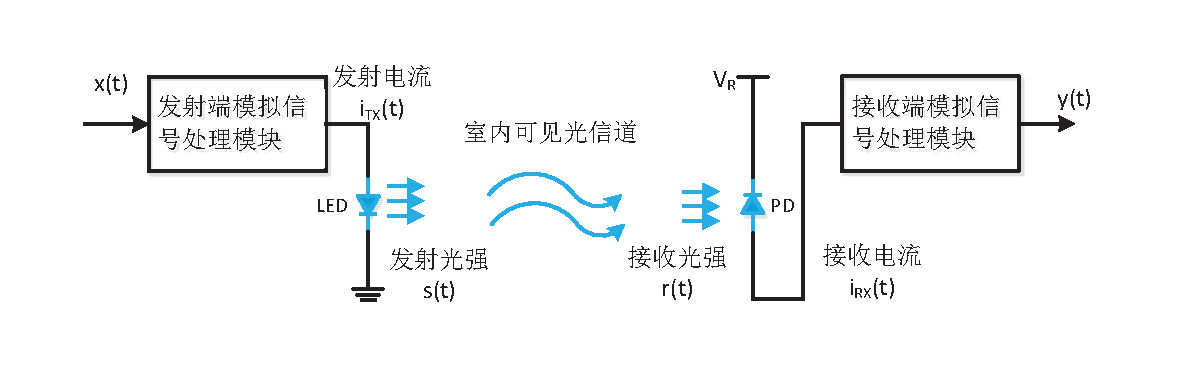
\includegraphics[width=\textwidth]{figures/chapter-2/BasicOpticalSystem.eps}
    \caption{光无线通信系统模型}
    \label{fig:BasicOpticalSystem}
\end{figure}
如\autoref{fig:BasicOpticalSystem}所示,在电信号域(Electrisity domain)发射端输出电压信号$x(t)$经过发光二极管后变成LED的电流$i_{TX}(t)$信号,接收端光敏二极管PD输出电流$i_{RX}(t)$,其最后转换成接收信号$y(t)$ ,在光信号域(Light Domain),首先在发射端发光二极管LED的电流信号$i_{TX}(t)$ 转变为发光强度$s(t)$,经过光信道后,在接收端光电二极管PD收到的光强信号为$r(t)$,经过光电转换,得到电流$i_{RX}(t)$。
所以在实际可见光通信系统中,信号传输由电光变换,光通道传输及光电变换三个过程组成,如\autoref{fig:BasebandModle}所示,接收端信号$y(t)$ 可以表示为:
\begin{equation}
    y(t)=x(t)\otimes h_1(t)\otimes h_2(t)\otimes h_3(t)+z(t)
\end{equation}
其中,$x(t)$表示发射端基带电压信号,$h_1(t)$表示电光转换系统的时域信道冲激响应(Channel Impose Response,CIR),$h_2(t)$表示可见光信道的时域信道冲激响应,$h_3(t)$表示光电转换系统的时域信道冲激响应
\cite{Yangxuecheng2015},
$z(t)$表示信道加性白高斯噪声(Additive White Gaussian Noise,AWGN),符从$z(t)\sim N(0,N_0/2)$分布,$N_0$为其功率谱密度,$\otimes$表示卷积运算。可见光通信系统的噪声,通常主要由热噪声和散弹噪声
\cite{Chenchunyan2014}。热噪声是一种高斯白噪声,在传统的射频无线通信系统中是很常见的。
散弹噪声也可以建模为白高斯噪声来处理,因为两个独立分布的高斯噪声还是高斯的,故我们可以将系统噪声统一建模为与信号独立的高斯白噪声。

\begin{figure}[htbp]
\centering
\includegraphics[width=0.9\textwidth]{figures/chapter-2/BasebandModle.eps}
\caption{光无线通信系统基带处理模型}
\label{fig:BasebandModle}
\end{figure}

\subsection{可见光通信系统信道特性}\label{subsection:Channel}
如\autoref{fig:BasebandModle}所示,可见光通信系统的信道由三部分组成,分别是电光转换信道$h_1(t)$、可见光空间自由传播信道$h_2(t)$ 和光电转换信道$h_3(t)$。因为用于可见光通信的LED具有优良的可调制性能,即存在一段线性区,而在实际设计光通信系统的时候,我力求LED 灯工作于线性区内,所以可以把$h_1(t)$当做线性信道来处理;光在自由空间传播时,光信号除了由直达径(Light of Sight, LOS)到达接收端之外,不可避免的还可以通过墙壁、家具反射径等非直达径(Non Light of Sight,Non-LOS)进入接收端,造成理论上的多径信道,并且由于光在自由空间传播的路径损耗正比于距离的四次方,及反射也会造成能量损耗,所以理论上$h_2(t)$是非线性的,但正由于路劲损耗与传播距离的四次方成正比,所以通过非直达径到达接收端的光信号能量远低于直达径的能量,考虑到这样的实际情况,故可以把光自由传播信号$h_2(t)$建模为线性信道;光电转换信道$h_3(t)$与电光转换信道$h_1(t)$类似,光电转换器件PD 也有一段线性区,只要设计系统时保证PD工作在线性区,也可以把$h_3(t)$ 建模为线性信道。由以上分析可得,组成可见光通信系统的三个组成部分都是线性的,那么整个信道也是线性的,其时域冲激响应可以表示为:
\begin{equation}
h(t)=h_1(t)\otimes h_2(t)\otimes h_3(t)
\end{equation}
\begin{figure}[htbp]
\centering
\includegraphics[width=0.9\textwidth]{figures/chapter-2/ChannelClass.eps}
\caption{光通信信道分类}
\label{fig:ChannelClass}
\end{figure}
\autoref{fig:ChannelResponse}所示为本课题对应硬件平台上通过发送伪随机序列(Pseudo-Noise Sequence,PN seq.)估计出来的信道响应(时钟200 MHz,PN码长度为16384),更加详细的信道估计理论将在第三章中介绍。其中图
\ref{fig:ChannelImpulseResponse}为时域冲激响应,幅度频率响应如图
\ref{fig:ChannelImpulseResponse-AmpFreqResponse}所示,相位频率响应见图
\ref{fig:ChannelImpulseResponse-PhsFreqResponse}。从
\ref{fig:ChannelImpulseResponse-AmpFreqResponse}可以看出可见光通信信道其实是一个低通系统。针对这样的信道特征,可以使用OFDM调制结合频域均衡技术来对抗频率选择性衰落,并且可以优化OFDM各子载波上的功率及比特分配,这部分内容将在第四章详细论述。
\begin{figure}[h]
    \centering
    \subfloat[室内可见光信道时域冲激响应]{
        \label{fig:ChannelImpulseResponse}
        \begin{minipage}[t]{1\textwidth}
            \centering
            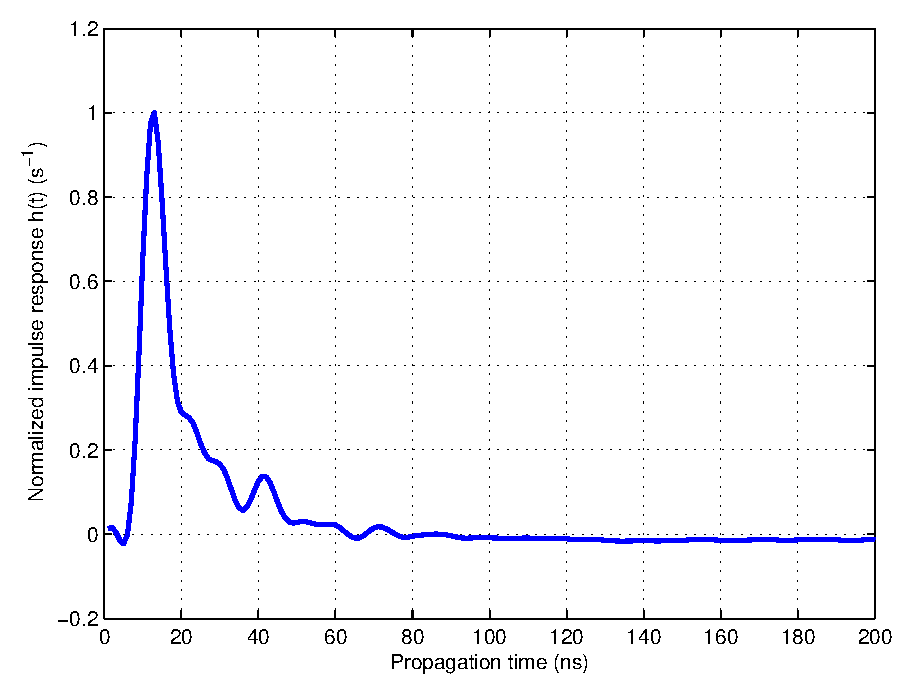
\includegraphics[width=0.6\textwidth]{figures/Chapter-2/ChannelImpulseResponse.eps}
        \end{minipage}
    }
    \par
    \centering
    \subfloat[室内可见光信道幅频特性]{
        \label{fig:ChannelImpulseResponse-AmpFreqResponse}
        \begin{minipage}[t]{0.5\textwidth}
            \centering
            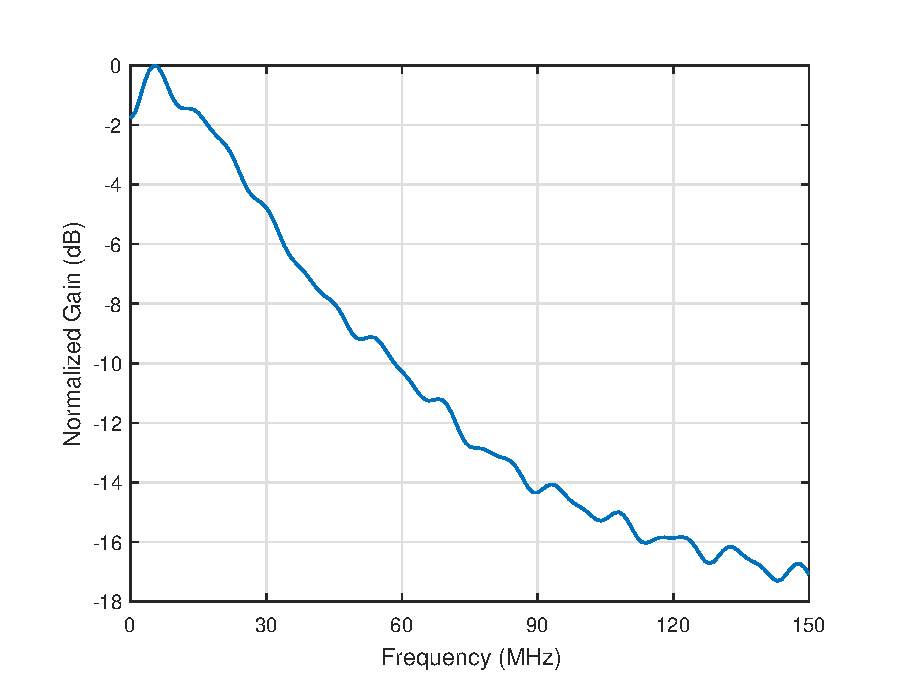
\includegraphics[width=\textwidth]{figures/Chapter-2/ChannelImpulseResponse-AmpFreqResponse.eps}
        \end{minipage}
    }
    \subfloat[室内可见光信道相频响应]{
        \label{fig:ChannelImpulseResponse-PhsFreqResponse}
        \begin{minipage}[t]{0.5\textwidth}
            \centering
            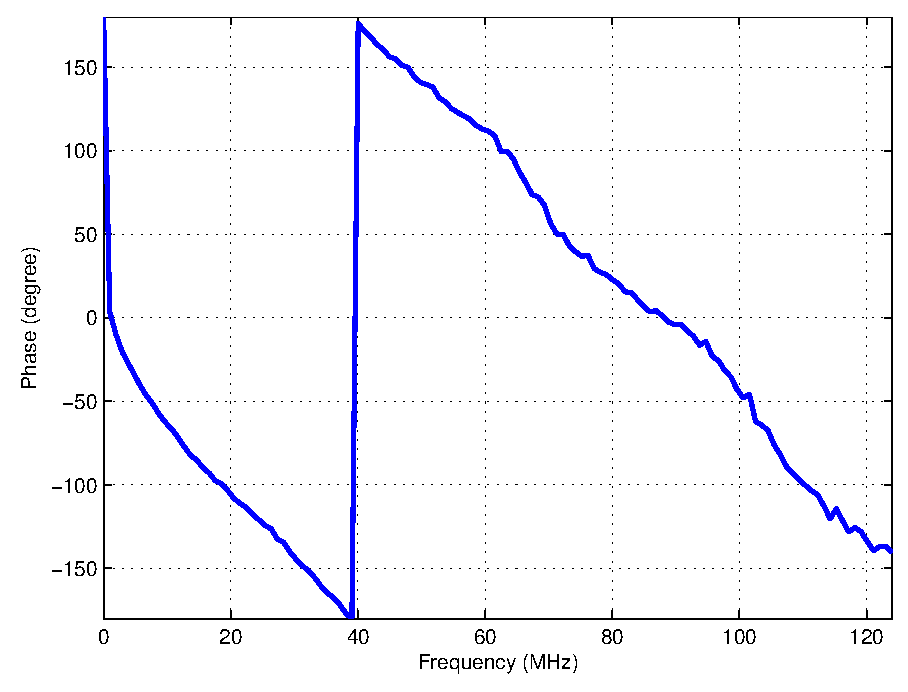
\includegraphics[width=0.97\textwidth]{figures/Chapter-2/ChannelImpulseResponse-PhsFreqResponse.eps}
        \end{minipage}
    }
    \caption{室内可见光信道的时频域响应特性}
    \label{fig:ChannelResponse}
\end{figure}

\subsection{光电元器件简介}
如前文所述,可见光通信与传统的无线通信最大的区别在于调制与信号检测上,射频无线通信必须把基带信号通过调幅、调频或者调相技术调制到高频率的载波上,在接收端再下变频得到基带信号。但目前可见光通信器件技术还不能直接去调制光的幅度、频率或者相位,而是使用发射端强度调制和接收端直接检测技术。在发射端,需要电光转换器件将电信号转换成光信号,在室内可见光通信中用到的主要是发光二极管LED,LED就是调制器,其工作线性范围是一个非常重要的指标,因为如果输入信号的动态变化范围较大,超出LED的线性调制范围,则会发生非线性失真,将严重影响通信性能,在可见光OFDM系统中尤其要注意这点,另外,LED 的响应时间是另一个重要指标,响应时间断的LED 能够被更高频率的信号调制,也就意味着带宽增加、通信速率增高。在接收端,需要光电转换器件将光信号再变成电信号以进行解调解码,目前大量使用的是光电二极管PD,光电二极管的PN结面积相对比较大,以便接收更多的入射光,其在反向电压的作用下,没有光照时,反向电流非常小,称为暗电流;在有光照时,反向电流急速增大,并且在一定范围内反向电流功率与光照强度成正比。本节将详细介绍发光二极管和光电二极管的通信特性。
\subsubsection{电光转换器件}
目前在光通信领域使用得电光转换器件主要有激光二极管(Laser Diode,LD)和发光二极管LED两类,这两种器件的性质差异很大,应用场景也不同。激光二极管响应速度非常快,但是线性区间非常小,几乎只有关闭和激发两种状态,而且发光角度较小,通信时需要发射端与接收端对准,所以一般用于高速光纤通信中。这里我主要讨论室内无线光通信使用的发光二极管LED。

发光二极管LED是一种掺杂了镓(Ga)、砷(As)和磷(P)等化合物的半导体器件,它跟普通的二极管一样,具有单向导电性,内部有PN节,P区含有多余的电子,N区则有多余得空穴。当给发光二极管加正向电压时,P区的高能电子与N区的空穴结合发生能级跃迁变为低能电子,根据能量守能,其将向外辐射电磁波,并且包含波长在380 nm到780 nm 之间的人眼可见的电磁波,具体辐射电磁波的波长主要由掺杂物的种类相关,这就是LED发光的基本原理。

\begin{figure}[htbp]
    \centering
    \subfloat[磷激发型LED光谱图]{
        \label{fig:OSTAR-Spectrum}
        \includegraphics[width=0.5\textwidth]{figures/chapter-2/LEUWS2LN-RelativeSpectralEmission.eps}
    }
    \subfloat[RGB三原色混光型LED光谱图]{
        \label{fig:RGB-Spectrum}
        \includegraphics[width=0.5\textwidth]{figures/chapter-2/LRTBR98G-RGB-RelativeSpectralEmission.eps}
    }
    \caption{两种白色LED光谱对比图}
    \label{fig:WhiteLED}
\end{figure}

众所周知,白光是一种混合光,故我们日常用于照明的白光LED灯发出的白光也是由几种光合成的。现在市面上的白光LED主要有两种类型。一种是磷光激发型,由蓝光LED激发荧光物质发出黄光,然后蓝光与黄光混合成我们人眼看到的白光;另一种是多色混合型,由多个LED发出不同颜色的光直接合成为白光,这种类型常见的红绿蓝(RGB)LED灯内部就含有三块晶片,分别发红光、绿光和蓝光。图\ref{fig:OSTAR-Spectrum}所示是德国OSRAM公司生产的磷光激发型发光二极管Lighting Plus LE UM S2LN的相对光谱分布图\cite{LE2011},图中峰值位于445 nm处的是蓝光LED发出的蓝色光波,而峰值位于555 nm处的是蓝光激发荧光物质产生的黄光。因为激发荧光物质发黄光的响应时间过长,在使用磷光型LED 进行可见光通信时,一般同时会在接收端加蓝色滤光片,滤掉响应过慢的黄光,所以虽然我们人眼看到的是白光,但是信号其实只调制在蓝光上,这就是前文中提到单色白光LED通信。图\ref{fig:RGB-Spectrum}所示多色混合型LED的相对光谱分布图\citep{LRTB2011},其具体型号为LRTB R98G,同为OSRAM 生产。图中可见红绿蓝三种色光的峰值分别位于635 nm、525 nm和465 nm 处,与林光激发型LED不同的是,红绿蓝三种色光分别由三种不同的LED晶片产生,都有很好的响应速度,我们可以对这三种色光分别调制,达到同时传输三路数据的目的,这样可以大大加大传输速率,即为前文所述的多色白光无线通信系统,也是本课题主要研究对象。


因为基于多色混合型LED的可见光通信系统能将各基色独立调制,总速率为各基色速率之和,所以相对于使用磷光激发型LED的单色光通信系统速率优势明显。现在也有专门的公司设计适合可见光通信的LED,如硅谷光擎(LED Engin),其生产了多种通信特性优异的多色混合型LED,如\autoref{fig:LED_LZ4_SputrcalPower} 所示为型号为LZC-03MA07的多色混合型LED的相对光谱功率分布和绝对光谱功率分布。从图\ref{fig:LED_LZ4_relativeSputrcalPower}中可以看出该白光LED 其由四种基色组成,分别为红(Red)、绿(Green)、蓝(Blue)和黄(Yellow),其中黄色有时也称为琥珀色(Amber),并且各基色光之间隔离明显,相互之间的干扰很少,同时图\ref{fig:LED_LZ4_absoluteSputrcalPower}说明各基色的发光功率相差明显,在设计多色光通信系统时也可以优化各个基色光发射功率,减少干扰,这个是我们后面研究的内容。
\begin{figure}[h]
    \centering
    \subfloat[LZC-03MA07相对光谱功率分布]{
        \label{fig:LED_LZ4_relativeSputrcalPower}
        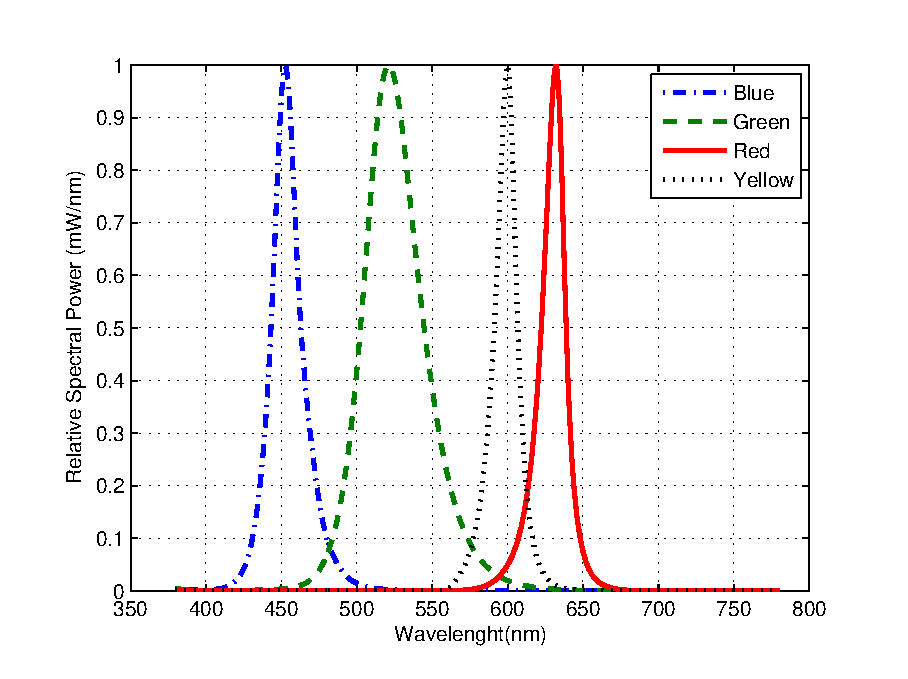
\includegraphics[width=0.5\textwidth]{figures/chapter-2/LED_LZ4_relativeSputrcalPower.eps}
    }
    \subfloat[LZC-03MA07绝对光谱功率分布]{
        \label{fig:LED_LZ4_absoluteSputrcalPower}
        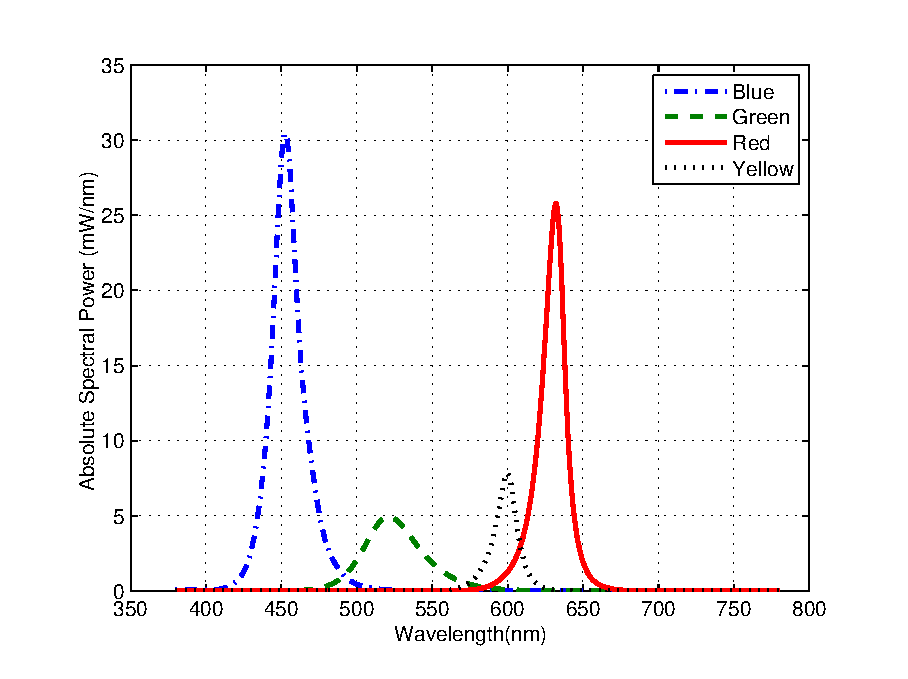
\includegraphics[width=0.5\textwidth]{figures/chapter-2/LED_LZ4_absoluteSputrcalPower.eps}
    }
    \caption{LZC-03MA07光谱功率分布}
    \label{fig:LED_LZ4_SputrcalPower}
\end{figure}

对于电光转换器件LED而言,我们除了要注意体面提到的线性范围和响应时间这两个指标之外,还要考虑LED的特性随温度的变化,如\autoref{fig:LZC_temprature} 所示\cite{LZC2013},图\ref{fig:LZC_relativeLightOuput}表明随着温度的升高,LED的输出光功率降低,但是各基色光功率降低的幅度不相同,其中黄光(Amber) 下降得最快,单温度升高到120 $^{\circ}$C时,输出功率降到常温下的20\%;而蓝光(Blue)受到的影响较小,功率输出变化不明显。受温度影响的还有各基色的主波长,主波长是指各基色光谱功率分布的峰值位置,如蓝光对应的是450 nm。如图\ref{fig:LZC_wavelengthShift}所示,也是黄光主波长变化最快,波长的漂移将导致接收端的滤光片效果降低,从而限制了总体的接收信噪比(Signal Noise Ratio, SNR)。故在设计可见光通信系统硬件时也要特别留意给LED散热,现在普遍的做法是将LED 安装在散热面积很大的金属灯头上。
\begin{figure}[h]
    \centering
    \subfloat[LZC-03MA07各基色相对输出光功率与温度的关系]{
        \label{fig:LZC_relativeLightOuput}
        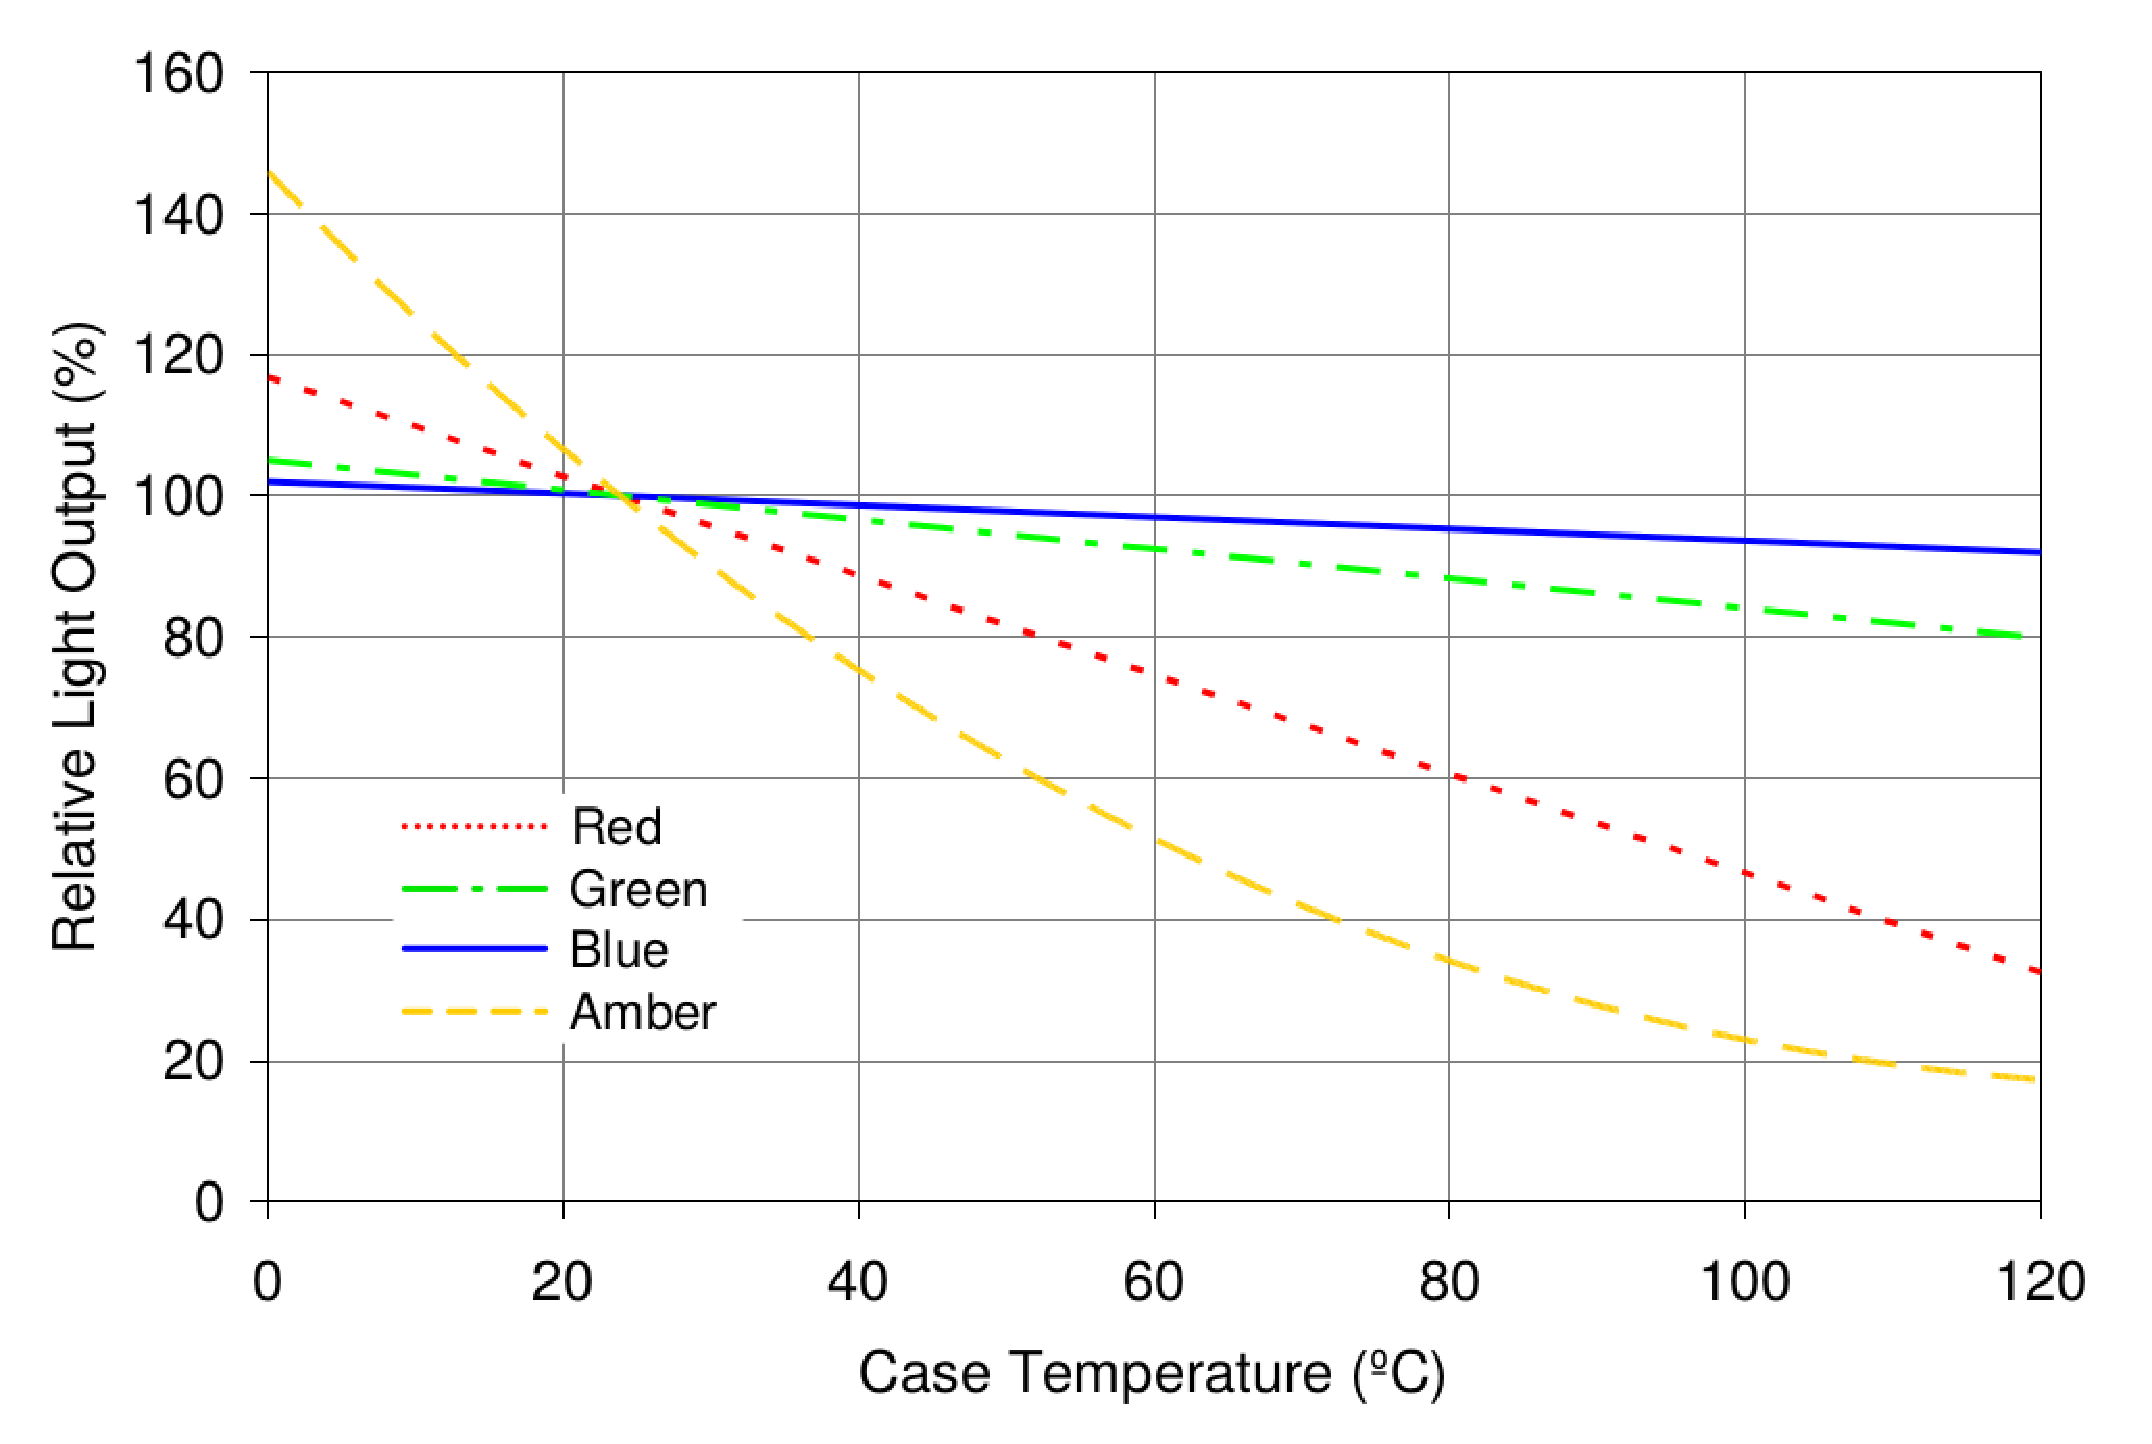
\includegraphics[width=0.5\textwidth]{figures/chapter-2/LED_Temperature_Light_Output.eps}
    }
    \subfloat[LZC-03MA07各基色主波长偏移量与温度的关系]{
        \label{fig:LZC_wavelengthShift}
        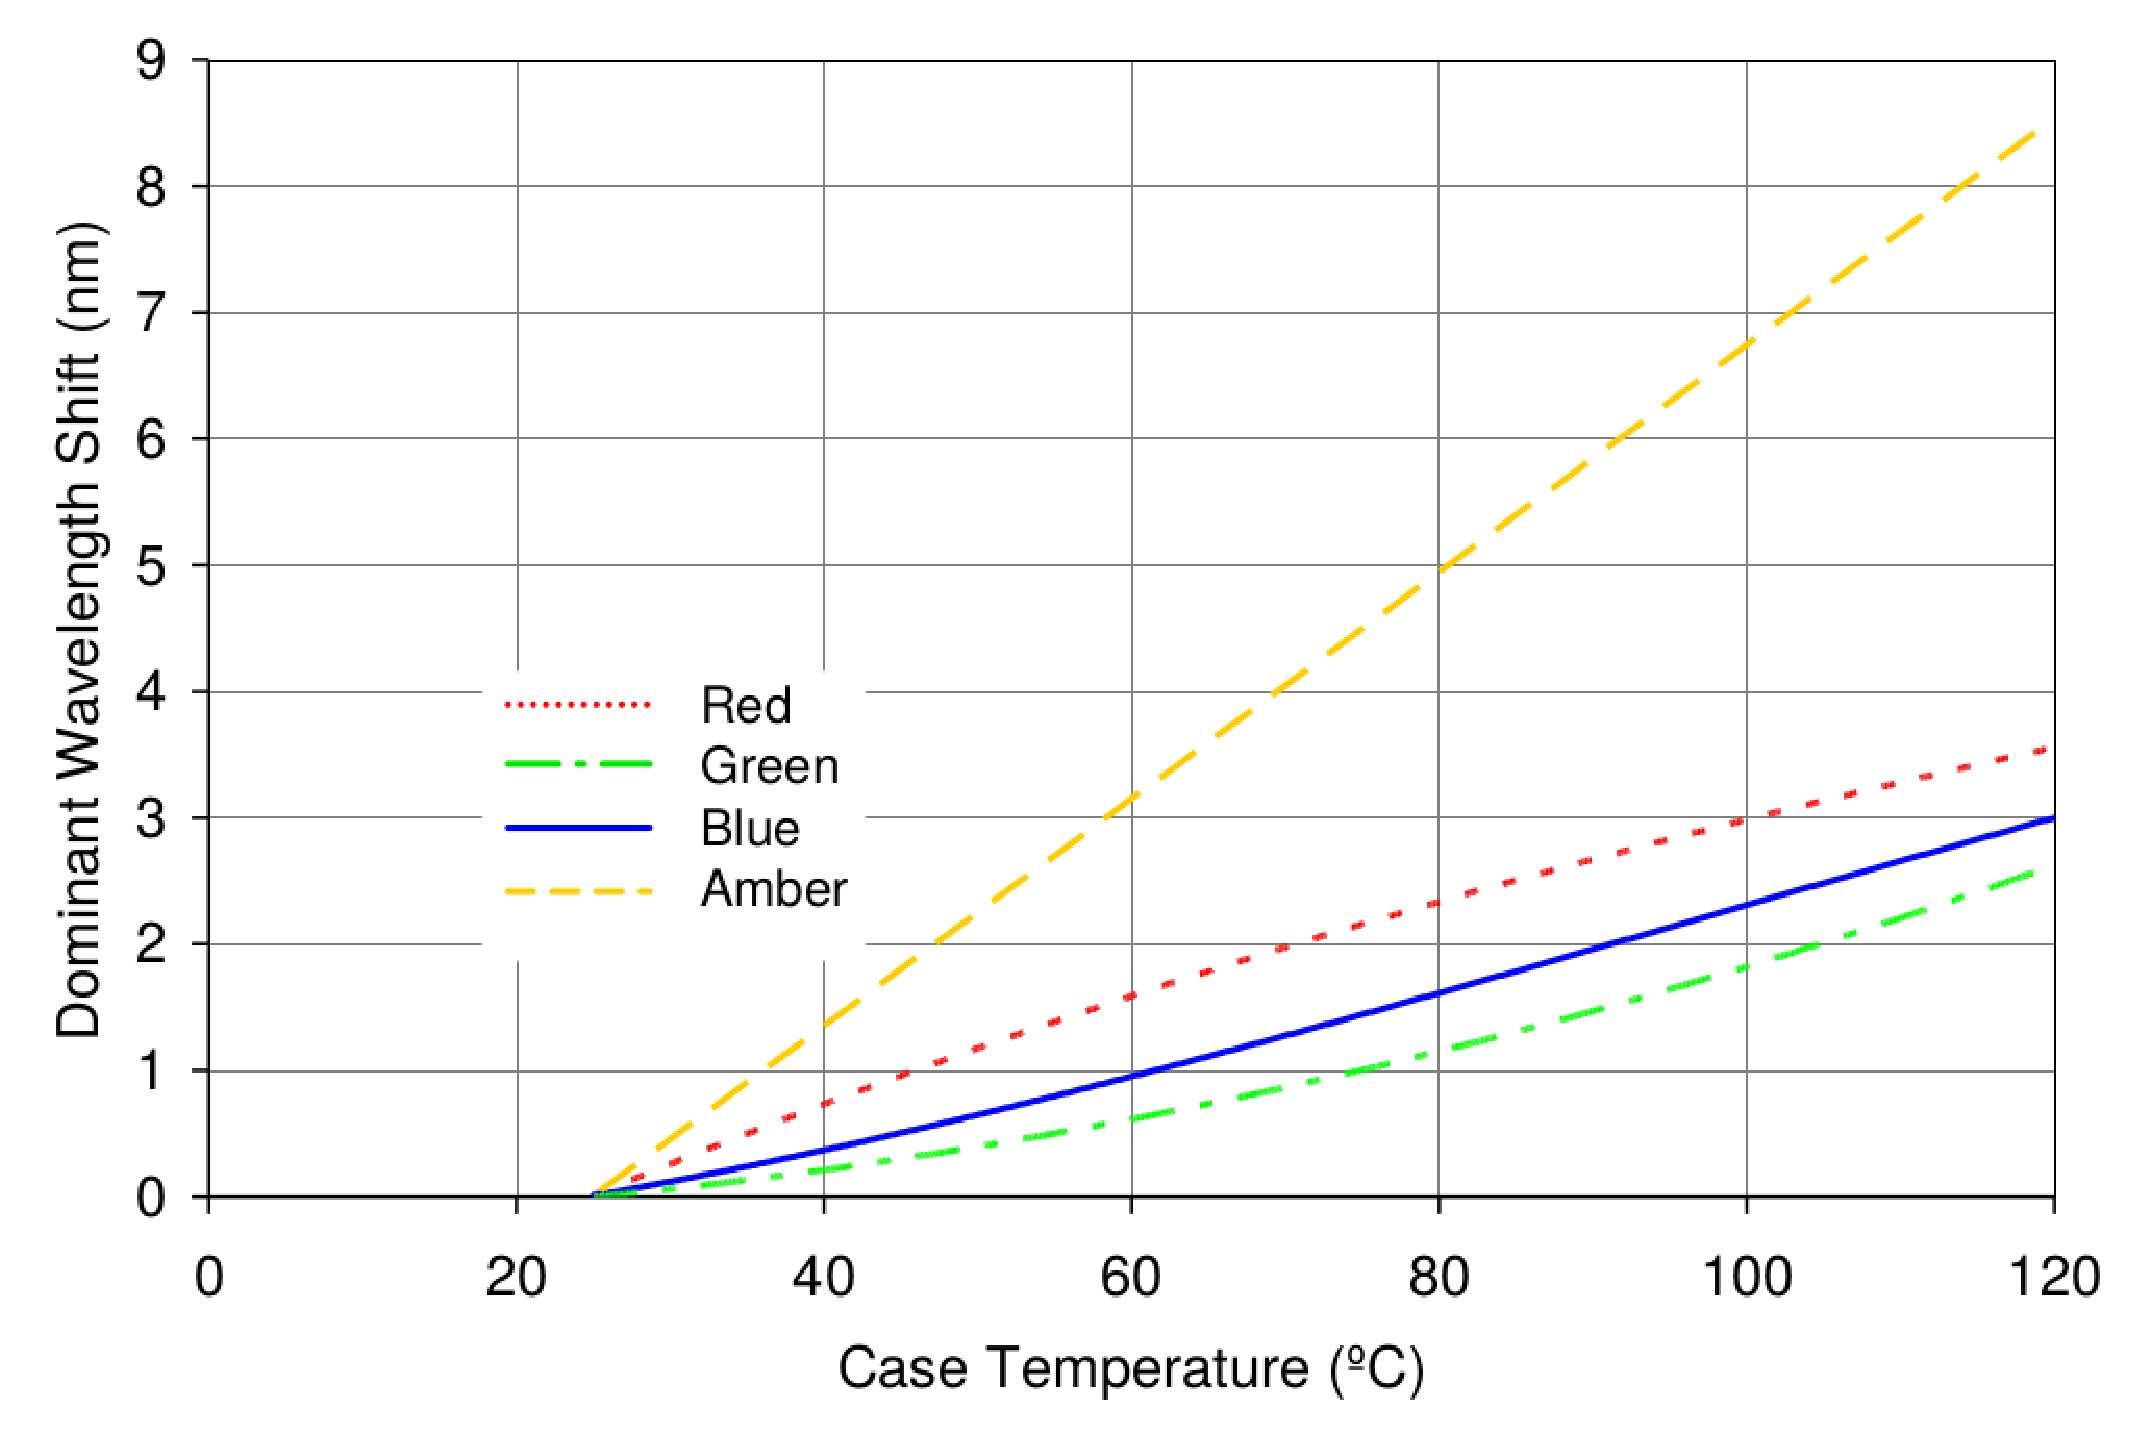
\includegraphics[width=0.5\textwidth]{figures/chapter-2/LED_Temperature_Wavelength_Shift.eps}
    }
    \caption{LZC-03MA07特性随温度变化关系}
    \label{fig:LZC_temprature}
\end{figure}

\subsection{光电转换器件}
现在使用最多的光电转换器件是光电二极管(PD)。光电二极管跟普通的二极管一样,也是一种含有PN节的半导体器件,只是会把PN节中的耗尽区通过某些方式暴露出来以接受光照。所谓耗尽区是在生产二极管时,在P区和N区交界的位置,N 区的电子会移向P 区并与空穴结合,这个P区与N区交界的区域就称为耗尽区。但是耗尽区不会持续增加,因为N 区的一个自由电子离开它的母体原子,原子就变成了正离子;同理,当自由电子进入P区并与其中的原子结合时,该原子就成为了负离子,离子形成电势阻止更多电子穿过耗尽区。在光电二极管中,耗尽区受到光照,由于光电效应,电子被激发,形成电子-空穴对,在方向配置电压的作用下形成反向电流,这就是光电二极管基本工作原理。
\begin{table}[htbp]
    \caption{PIN 与 APD光电二极管对比}
    \label{tab:PIN_APD_Comparsion}
    \centering
    \begin{tabular}{lllll}
        \toprule
         & PIN & APD \\
        \midrule
        光电增益       & 一般   &雪崩效应    \\
        调制带宽       & 最高几百MHZ  &最高几十GHZ    \\
        线性动态范围   & 较宽  &较窄    \\
        温度敏感度    & 不敏感  &敏感    \\
        制作工艺    &简单 &复杂    \\
        价格    & 低  &高    \\
        \bottomrule
    \end{tabular}
\end{table}

目前在可见光通信中应用的光电二极管有PIN型和雪崩型(Avalanche photodiode,APD)两种,PIN型光电二极管就是在普通的光电二极管的P区和N区之间加入了低掺杂度的I 区,使得耗尽区变厚了,从而缩短了其响应时间,并且提高了截止频率,其调制带宽可达数百兆赫兹,能够适应高速通信系统的要求。同时PIN 型二极管还有线性范围宽、制作工艺简单及价格低等优点。雪崩型光电二极管比较特殊,它的工作原理是在其P区和N 区两端加了反向高电压,当有光照射耗尽区产出自由电子和空穴时,在反向高压的作用下,电子和空穴高速碰撞晶格原子,产生更多的电子和空穴,此过程像“雪崩”一样继续下去,从而产生了很大的反向电流。雪崩型光电二极管的优点是灵敏度高、增益高及带宽高,但是制造工艺复杂,价格较贵。PIN型和雪崩型光电二极管的比较如下表\ref{tab:PIN_APD_Comparsion}所示。


\subsection{滤光片}
如前所述,在使用磷光激发型LED的单色光通信系统中,我们要滤掉响应时间过长的黄光只取携带信息蓝光;在使用多色混合型LED 的多色光通信系统中,我们要在每个基色上调制信息,在接收端要把每个基色分别提取出来进行数字信号处理。这些过程要需要一个光学元件——滤光片,准确来说应该是带通滤光片。带通滤光片只允许较窄波长范围的光通过,常见的是法布里-珀罗型滤光片,它实质 上是一个法布里-珀罗标准具(见法布里-珀罗干涉仪)。具体结构为:玻璃衬底上涂一层半透明金属层,接着涂一层氟化镁隔层,再涂一层半透明金属层,两金属 层构成了法布里- 珀罗标准具的两块平行板。当两极的间隔与波长同数量级时,透射光中不同波长的干涉高峰分得很开,利用别的吸收型滤光片可把不允许透过的光 滤掉,从而得到窄通带的带通滤光片,其通频带宽度远比普通吸收型滤光片要窄\cite{OpticalFilter}。
\begin{figure}[htbp]
    \centering
    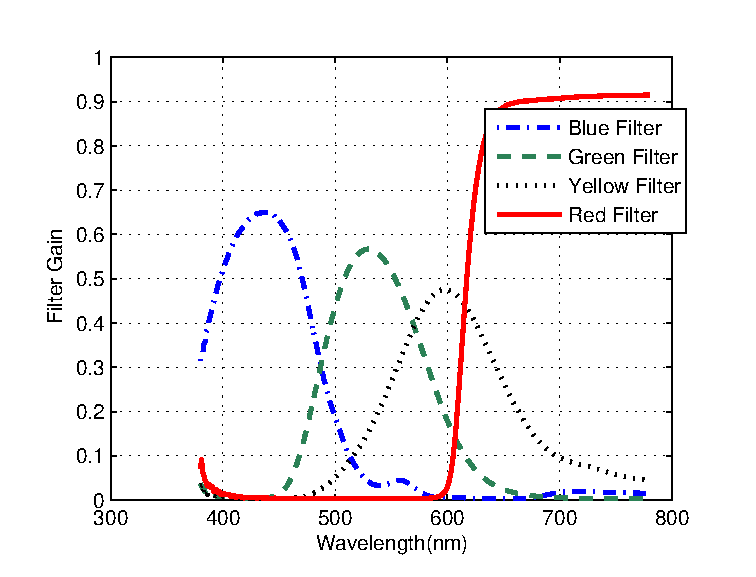
\includegraphics[width=0.8\textwidth]{figures/Chapter-2/MulticolorFilterGain.eps}
    \caption{滤色片滤色性能}
    \label{fig:MulticolorFilterGain}
\end{figure}
类型于滤波器对于射频无线通信的作用,滤光片也对可见光通信系统的性能有着重要的影响,但是精密的滤光片虽然性能优良,但制造工艺复杂、价格昂贵,不利用可见光通信技术的推广,所以在可见光通信中一般会选择价格一般但性能稍差的滤波片,然后借助数字信号处理技术来弥补滤光片性能的不足。本课题搭建的硬件平台发射端使用的是前面提到的混合型LED——LZC-03MA07,接收端使用四块滤光片滤出四个基色,分别是蓝光滤光片DTB435、绿光滤光片DTB530、黄光滤光片DTB600和红光滤光片HB610,它们的滤光带通增益如
\autoref{fig:MulticolorFilterGain}所示,其中除红光滤光片是低通滤光片外(对频率而言),其他三个都是带通的,各滤光片对光信号都有一些衰减,其中黄光滤光片的衰减最大,并且各色之间都有一些串扰。
\autoref{fig:MultiColorReceiveredFilter}所示是接收端未加滤光片接收信号和由四个经滤光片提取的四个基色组合的光功率的比较,可以更清楚地看出滤光片的功能和对信号的衰减。
\begin{figure}[htbp]
    \centering
    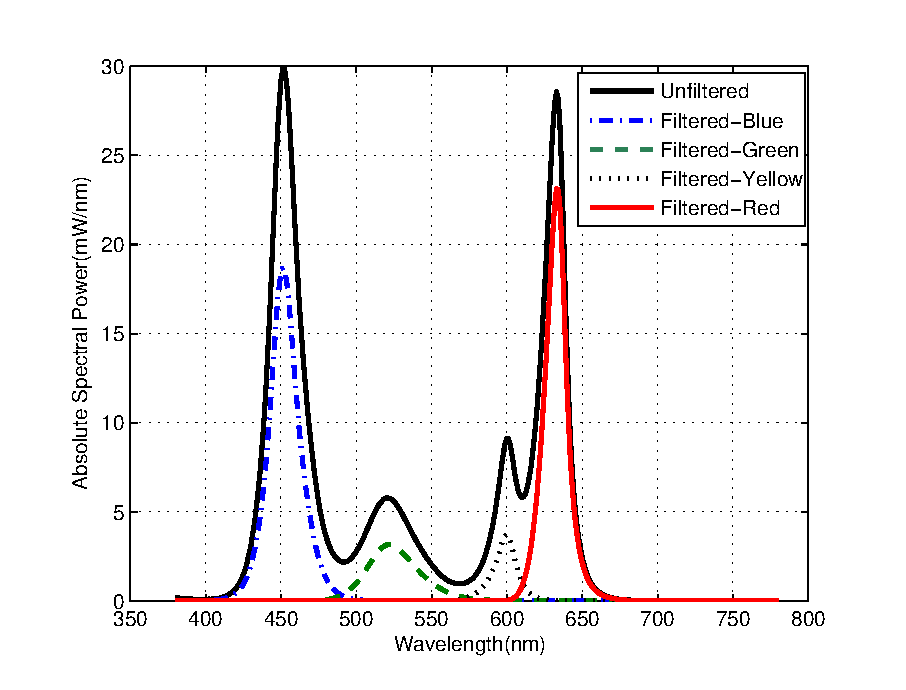
\includegraphics[width=0.8\textwidth]{figures/Chapter-2/MultiColorReceiveredFilter.eps}
    \caption{接收端滤色后光功率谱}
    \label{fig:MultiColorReceiveredFilter}
\end{figure}
\section{OFDM技术在室内可见光通信中的应用}
\subsection{OFDM技术发展历程}
正交频分复用(OFDM)是一种多载波调制技术,是一种能有效地对抗频率选择性衰落途径,而且频谱利用率较高,实现简单,在很多现代通信系统中得到了广泛的应用,如DSL、WIFI及LTE等。OFDM技术发展历程及其应用如
\autoref{fig:HistoryOfOFDM}所示,最早由美国贝尔实验室的Chang 在1966 申请的专利“正交频分复用数字传输系统”提出;1969年,Salz和Weinstein研究了使用傅里叶变换来实现OFDM的通信系统;用来抵抗码间干扰的循环前缀(Cyclic Prefix, CP)于1980年加入OFDM系统。这是OFDM 技术理论发展最重要的三个节点
\cite{armstrong2009ofdm}。在上世纪80年代中期,人们开始研究OFDM技术在实际通信系统中的应用,1985年,同样来自贝尔实验室的Cimini研究了OFDM用于移动通信的可能性;1987年, Lassalle 和 Alard将OFDM技术推广到无线广播系统,并且揭示了前向纠错编码和OFDM技术结合的重要性,对于广播通信工程师而言,OFDM技术也称为C-OFDM(Coded OFDM);最先提出在有线通信中使用OFDM技术的是来自斯坦福大学的Cioffi等人,同时他们展示了OFDM可以作为数字用户线路(Digital Subscriber Line, DSL)的一种替代调制方式;如绪论所述,OFDM近年来也开始被应用于光通信中,根据在时序信号要不要加直流偏置可以把光OFDM 分为直流偏置光OFDM调制方式(DC-biased optical OFDM,DCO-OFDM)和非对称光OFDM调制方式(Asymmetrically-clipped optical OFDM, ACO-OFDM)两种,下面简要介绍这两种光OFDM 调制技术。
\begin{figure}[htbp]
    \centering
    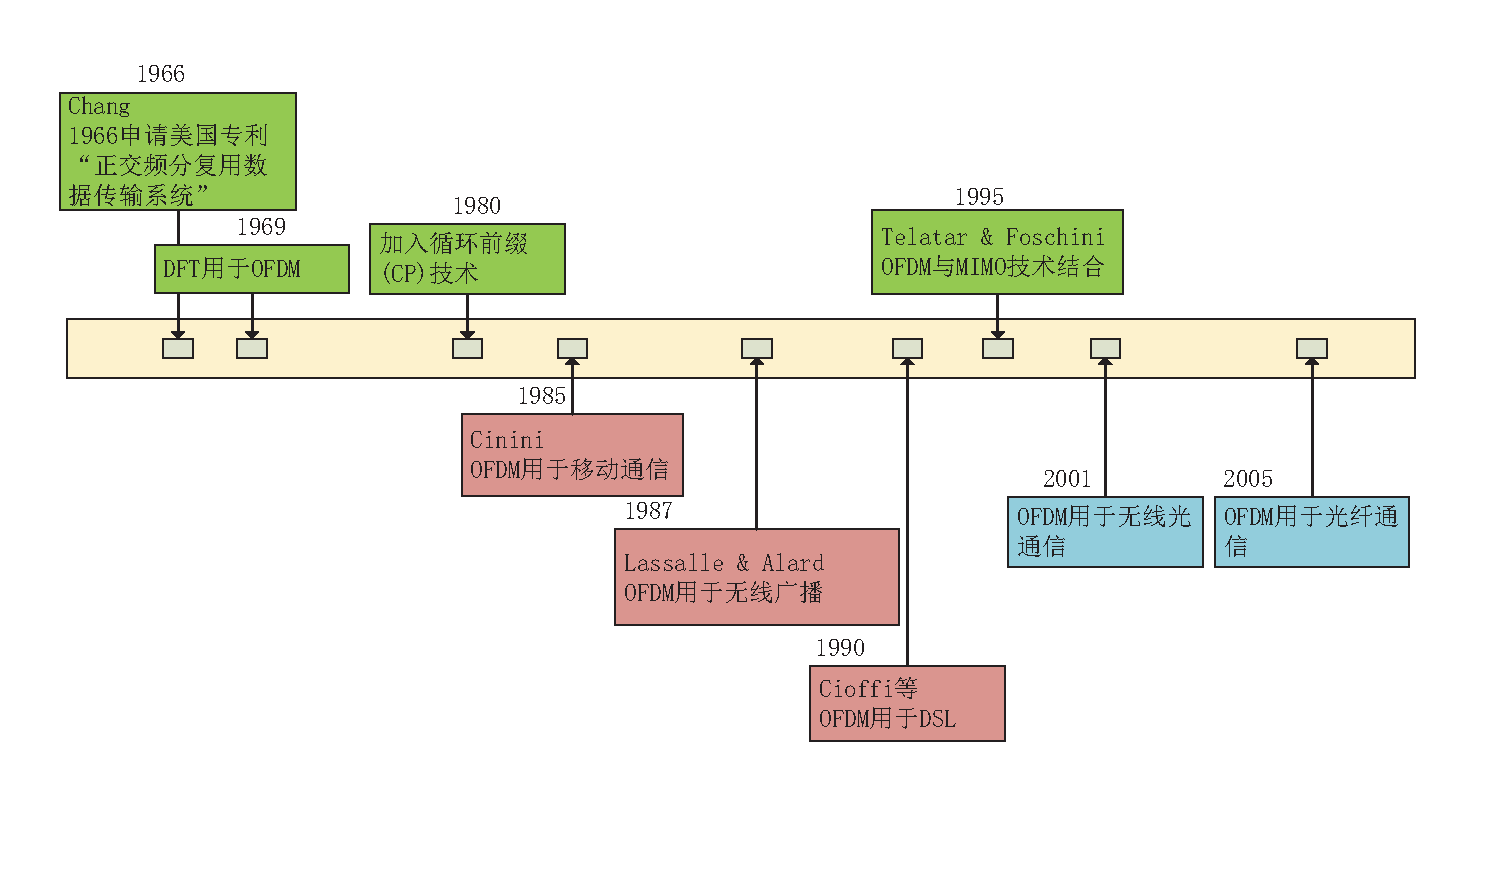
\includegraphics[width=0.8\textwidth]{figures/Chapter-2/HistoryOfOFDM.eps}
    \caption{OFDM技术发展历程及其应用}
    \label{fig:HistoryOfOFDM}
\end{figure}
\subsection{DCO-OFDM简介}
\begin{figure}[htbp]
    \centering
    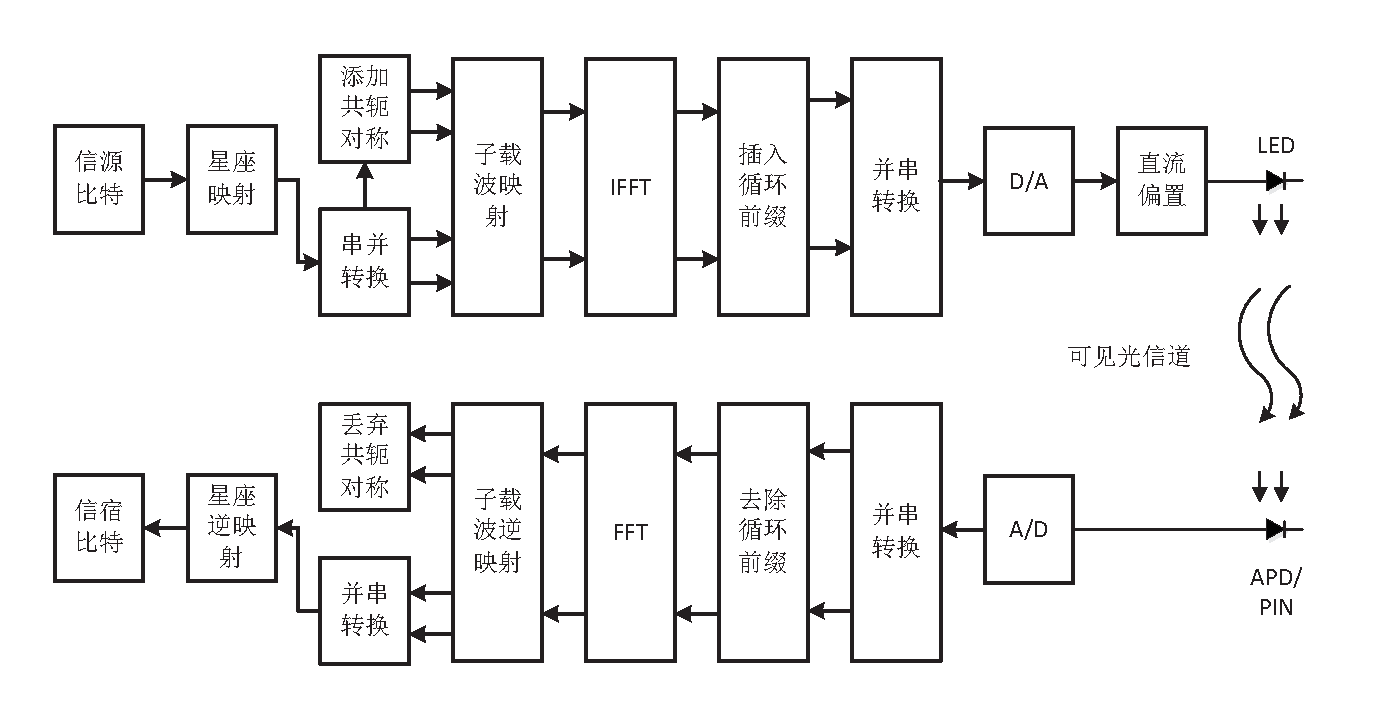
\includegraphics[width=0.9\textwidth]{figures/Chapter-2/DCO-OFDMStructure.eps}
    \caption{DCO-OFDM流程图}
    \label{fig:DCO-OFDMStructure}
\end{figure}

DCO-OFDM调制技术原理框图如\autoref{fig:DCO-OFDMStructure} 所示。因为在光通信中,现在使用的都是强度调制,直接检测技术,所以要保证LED灯输入信号是实数。为了满足这个条件,我们要将逆傅里叶变换(Inverse Fast Fourier Transform, IFFT)之前的频域复信号设计为满足共轭对称的形式\cite{proakisdigital},假设我们使用的子载波数目为$N/2$,待发送的复信号为$X(k),k = 0, 1, 2, \cdots, N/2-1$,则其对应的共轭对称形式为:
\begin{equation}
    \tilde{X}(k) =
    \begin{cases}
        \Re\{X(0)\}  & k = 0 \\
        X(k) & k = 1, 2, \cdots, N/2-1 \\
        \Im\{X(0)\} & k = N/2 \\
        X^*(N-k) & k = N/2+1, \cdots, N-1
    \end{cases}
    \label{equ:HermitianSymmetry}
\end{equation}
其中$N$为FFT长度,“$\Re\{\cdot\}$”表示取实部,“$\Im\{\cdot\}$”为取虚部,“$(\cdot)^*$”代表做共轭运算。现在我们对满足共轭对称的信号$\tilde{X}(k),k=0,1,...,N-1$ 做$N$点IFFT运算,得到时域信号表达式为:
\begin{equation}
    x(n) = \frac{1}{\sqrt{N}}\sum \limits_{k=0}^{N-1}\tilde{X}(k)e^{\frac{j2\pi kn}{N}}
    \label{equ:DCO_OFDM_Sig}
\end{equation}
在式\ref{equ:DCO_OFDM_Sig}中,取任意$k$,假设$X(k)=a+bj$,则$X(N-k)=a-bj$,则有:
\begin{align}
    T(k) &= X(k)e^{\frac{j2\pi kn}{N}}+X(N-k)e^{\frac{j2\pi (N-k)n}{N}}\nonumber  \\
    &=\sqrt{a^2+b^2}e^{\frac{j2\pi kn+j\theta}{N}}+\sqrt{a^2+b^2}e^{-\frac{j2\pi kn+j\theta}{N}}\nonumber \\
    &=2\sqrt{a^2+b^2}\cos(\frac{2\pi kn}{N}+\theta)
    \label{equ:DCO_OFDM_Proof}
\end{align}
其中$\theta$表示$X(k)$的幅角,由式\ref{equ:DCO_OFDM_Proof}知$T(k)$必为实数,那么:
\begin{equation}
    x(n)=\frac{1}{\sqrt{N}}(\sum \limits_{k=1}^{N/2-1}T(k)+ \Re\{X(0)\} +\Im\{X(0)\}(-1)^n)
\end{equation}
说明IFFT之后输出的时域信号确实为实信号。作为LED强度调制信号,还要满足正数这个条件,而共轭对称后输出的结果虽然已是实数,但是有正有负,为了使其变为正数,我们可以在改实数信号上加一个直流正偏置,但是这个偏置选择也非常讲究,如果偏置过低,则会造成下削波,而过高则会让LED进入非线性区。在实际系统设计时,要根据IFFT输出时域信号的统计情况要决定偏置大小。DCO-OFDM 加偏置后的时域信号如图\autoref{fig:DCO-OFDMSignal}所示。

\subsection{ACO-OFDM调制}

\begin{figure}[h]
    \centering
    \includegraphics[width=0.9\textwidth]{figures/Chapter-2/ACO-OFDMStructure.eps}
    \caption{ACO-OFDM流程图}
    \label{fig:ACO-OFDMStructure}
\end{figure}
DCO-OFDM技术实现简单、频谱利用率高,但是有个缺点就是要加直流偏置,这样降低了其能效效率。ACO-OFDM就是在DCO-OFDM的基础上发展而来的另一种光OFDM 结构,解决要加直流偏置的问题。ACO-OFDM主要是利用IFFT的一个性质,即只在奇数子载波上调制数据,偶数子载波置为0,同时让复信号满足共轭对称性,这样的频域复信号得到的时域实信号满足一个$x(n+N/2)=-x(n)$这样的平移$N/2$ 反对称特性,利用这样的特性,在发射端不需要加偏置,而是直接进行零值削波,在接收端也能正确解调出信息,其原理框图如
\autoref{fig:ACO-OFDMStructure} 所示。下面先简要证明其平移反对称特性。

如前所述,ACO-OFDM要将所有的偶数子载波的数据置为零,即不用偶数子载波,所以其频谱利用率只有DCO-OFDM的一半。假设OFDM 待调制复信号为$X(k),k=0,1,2,\cdots,N/4-1$,将偶数子载波置为零,同时满足共轭对称性,得到IFFT频域信号为:
\begin{equation}
    \tilde{X}(k) =
    \begin{cases}
        0 & \text{k为偶数} \\
        X(\frac{k-1}{2}) & k = 1, 3, 5, \cdots, N/2-1 \\
        X^*(\frac{N-1-k}{2}) & k = N/2+1, N/2+3, \cdots, N-1
    \end{cases}
    \label{equ:ACO_OFDM_Freq}
\end{equation}
因为 $\tilde{X}(k)$满足共轭对称性,则其IFFT输出首先一定会是实数,又因为:
\begin{equation}
    x(n+N/2) = \frac{1}{\sqrt{N}}\sum \limits_{k=0}^{N-1}\tilde{X}(k) e^{j\frac{2\pi k(n+N/2)}{N}} = \frac{1}{\sqrt{N}} \sum \limits_{k=0}^{N-1} (-1)^k\tilde{X}(k)e^{j\frac{2\pi kn}{N}}
    \label{equ:ACO_OFDM_equ1}
\end{equation}
其中偶数子载波上的信号被置为零,所以\label{equ_ACO_OFDM_equ1} 可以化简为:
\begin{equation}
    x(n+N/2) = -\frac{1}{\sqrt{N}} \sum \limits_{k=0}^{N-1} \tilde{X}(k)e^{j\frac{2\pi kn}{N}} = -x(n)
\end{equation}
即平移反对称性成立。利用这个特性,发射端可以进行零值削波,即将负值时域信号置为0,正值信号值不变,然后用这个削波后的信号去调制LED,下面证明考虑无噪声的情况下接收端能正确恢复信号。
由傅里叶变换:
\begin{equation}
    X(m) = \frac{1}{\sqrt{N}}\sum \limits_{k=0}^{N-1}x(k)e^{-\frac{j2\pi km}{N}}
    \label{equ:FFT}
\end{equation}
式\ref{equ:FFT}可以改写为:
\begin{align}
\label{equ:ACO_OFDM_Proof1}
    X(m) = &\frac{1}{\sqrt{N}}\sum \limits_{k=0, x(k)>0}^{N-1}\left(x(k)e^{-\frac{j2\pi km}{N}}+x(k+\frac{N}{2})e^{-\frac{j2\pi (k+\frac{N}{2})m}{N}}\right)\nonumber \\
         &+\frac{1}{\sqrt{N}}\sum \limits_{k=0, x(k)<0}^{N-1}\left(x(k)e^{-\frac{j2\pi km}{N}}+x(k+\frac{N}{2})e^{-\frac{j2\pi (k+\frac{N}{2})m}{N}}\right) \nonumber\\
\end{align}
因为偶数子载波上值全为零,只有奇数子载波上有非零值,则式\ref{equ:ACO_OFDM_Proof1}中第一个和式的第二部分与第一部分相等,同样第二个和式的第二部分与第一部分也相等,则\ref{equ:ACO_OFDM_Proof1}可以写为:
\begin{equation}
X(m) = \frac{2}{\sqrt{N}}\sum \limits_{k=0, x(k)>0}^{N-1}(x(k)e^{-\frac{j2\pi km}{N}}) + \frac{2}{\sqrt{N}}\sum \limits_{k=0, x(k)<0}^{N-1}(x(k)e^{-\frac{j2\pi km}{N}})
\label{equ:ACO_OFDM_Proof2}
\end{equation}
又由于对于已削波的信号,式\ref{equ:ACO_OFDM_Proof1} 中第一个和式的第二部分和第二个和式的第一部分都为零,故得:
\begin{equation}
X_{c}(m)=\frac{1}{\sqrt{N}}\sum \limits_{k=0}^{N-1}x_{c}(k)e^{-\frac{j2\pi km}{N}}=\frac{X(m)}{2}
\label{equ:ACO_OFDM_Proof3}
\end{equation}
式中$x_c(k)$,$X_c(m)$分别表示在不考虑任何噪声情况下接收端的时域信号和频域信号,可知接收到的频域信号为发射的频域信号的一半,也就是说成比例的,而这个比例系数可以在信道估计中很容易估计得到,所以ACO-OFDM在原理上是成立的。

\begin{figure}[h]
    \centering
    \subfloat[DCO-OFDM信号]{
        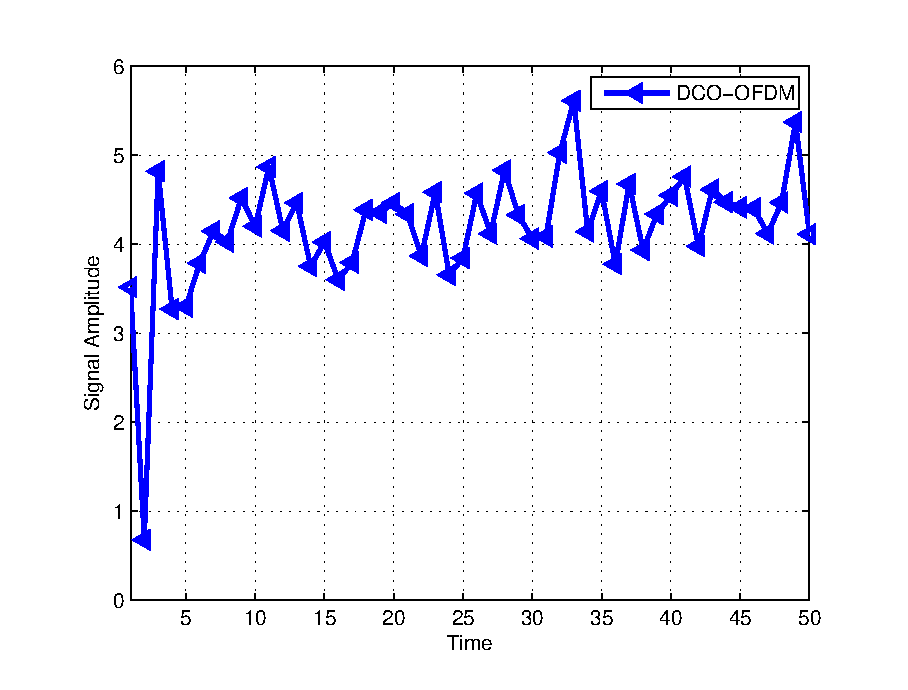
\includegraphics[width=0.5\textwidth]{figures/Chapter-2/DCO-OFDMSignal.eps}
        \label{fig:DCO-OFDMSignal}
    }
    \subfloat[ACO-OFDM信号]{
        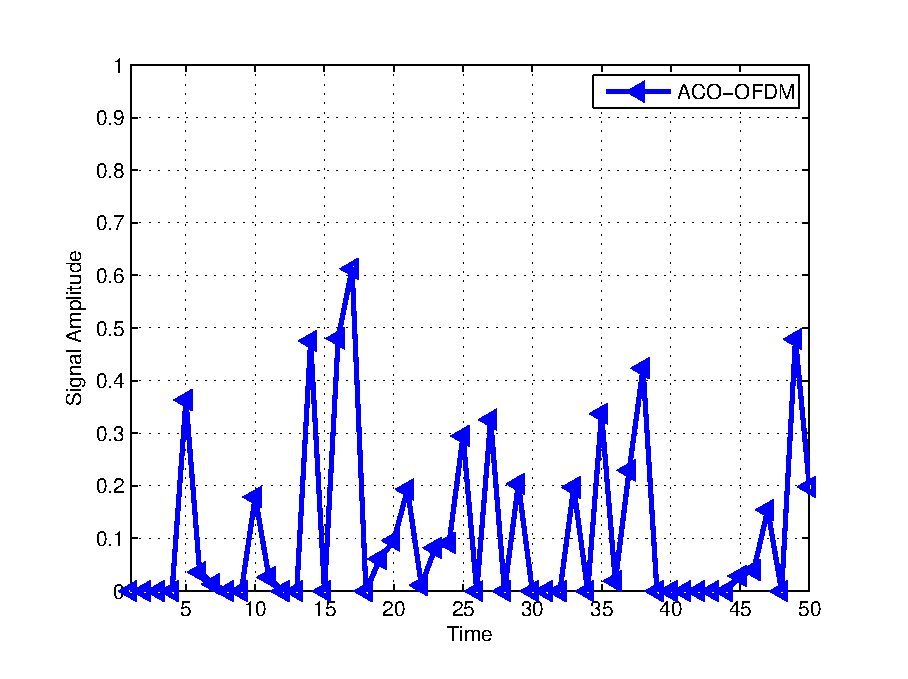
\includegraphics[width=0.5\textwidth]{figures/Chapter-2/ACO-OFDMSignal.eps}
        \label{fig:ACO-OFDMSignal}
    }
    \caption{DCO-OFDM信号调与ACO-OFDM信号比较}
    \label{fig:DCO-OFDMVSACO-OFDM}
\end{figure}
\section{本章小结}
本章首先可见光通信的基本原理,包括系统模型、信道特征及光电元器件等,本文联系实际情况将可见光通信信道建模为线性信道,然后介绍了电光转换器件LED,详细说明了荧光激发型LED和多色混合型LED的工作原理和特性,还介绍PIN 和APD两类光电转换器件及接收端使用的滤光片。理解这些光电元器件的原理与作用有益于理解整个可见光通信系统。由于OFDM调制技术非常适应光低通信道,在可见光通信中也得到了广泛的使用,所以本章也介绍了光OFDM技术,主要说明了DCO-OFDM和ACO-OFDM的工作原理及区别。

   % % !Mode:: "TeX:UTF-8"
\chapter{可见光多波段OFDM系统的信道估计}
\section{引言}
所谓信道估计,就是在接收端估计出信道状态信息(Channel State Information,CSI),为下一步地解调做准备,也是自适应传输技术的基础。无线通信一个重要的特征就是发射端到接收端之间的路径比较复杂,不像有线通信那样是固定且可预知的,所以信道估计技术在无线通信领域格外重要,特别是在OFDM 等需要相干检测的系统中。本章将着重介绍信道估计技术,首先介绍传统射频通信中OFDM 系统的信道估计方法,然后具体到可见光通信系统中的信道估计问题,再将结合实际系统设计,讨论信道的非线性问题,最后将研究多色可见光通信系统中各波段之间串扰的估计。
\section{OFDM信道估计常用方法}
信道估计总体可以分为两大类,盲信道估计和基于导频的信道估计。盲信道不需要额外的导频或者训练序列,因此频率利用率高;但是它的缺点是计算量大、算法复杂,而且精度低、收敛速度缓慢,难以用于移动通信环境
\cite{石钧2012ofdm}。基于导频的信道估计原理是在发射端插入专门用于信道估计的导频或者训练序列,并且这些序列对于接收端也是已知的,接收端根据接收到的经过了信道后的导频序列与原导频序列之间的关系,估计出信道冲击响应(Channel Impulse Response,CIR)。这类信道估计方法因为要插入导频序列会稍微降低整个系统的传输速率,但是其估计实现复杂度低、估计精度高,在实际工程中大都采用这种方法。本节也主要讨论基于导频的信道估计算法。
\begin{figure}[htbp]
    \centering
    \subfloat[块状导频放置方式]{
        \label{fig:BlockTypePilot}
        \includegraphics[width = 0.5\textwidth]{figures/chapter-3/BlockTypePilot.eps}
    }
    \subfloat[梳状导频放置方式]{
    	\label{fig:CombTypePilot}
        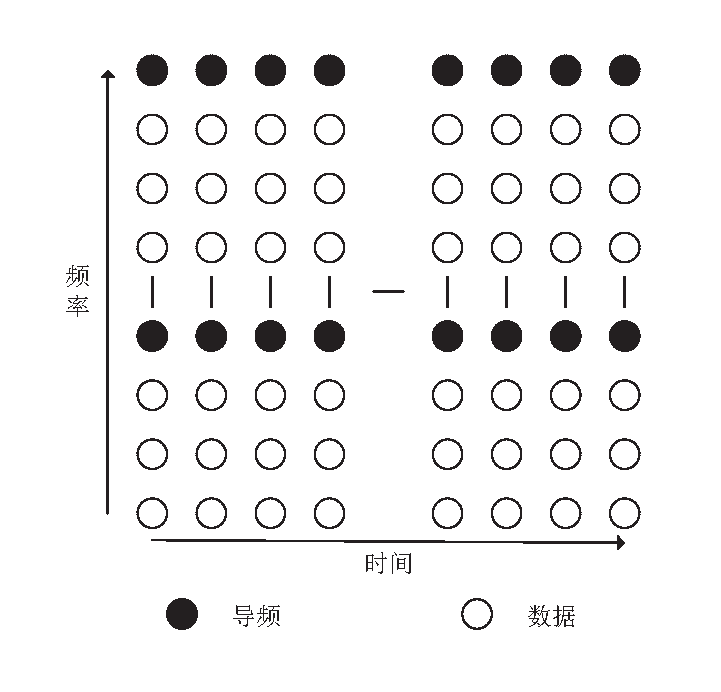
\includegraphics[width = 0.5\textwidth]{figures/chapter-3/CombTypePilot.eps}
    }
    \caption{导频放置方式}
    \label{fig:PilotAllocation}
\end{figure}
对于基于导频的信道估计而言,研究人员对其导频放置方式也进行了深入的研究,如\autoref{fig:PilotAllocation}所示,常见的有块状和梳状两种放置方式。

块状导频放置方式见图\ref{fig:BlockTypePilot},它的导频序列连续放置在一个OFDM符号上,但是在时间上不是连续的,也就是说要隔若干个OFDM符号才放置一个导频序列。在工程实现中,更常见的一种情况是导频序列即用于信道估计,又用于同步,这样一般是一帧放置一个导频符号。块状导频放置方式的优点是结构简单,计算复杂度低,但是因为要隔一段时间才估计一次信道,所以块状导频放置方式一般用于信道时变比较缓慢的信道。

梳状导频放置方式如图\ref{fig:CombTypePilot}所示,在每个OFDM符号上,它只选择在特定的子载波上放置导频序列,而其他子载波上放置数据符号,并且每个OFDM符号的结构都是如此。它的工作原理是先估计出放置了导频的子载波处的信道响应,然后根据这些信道响应通过插值的方式得到那些放置了数据符号的子载波处的信道响应。它的优点是每个符号都会估计信道,能够应对快速时变的信道,但是它要使用插值计算,所以复杂度比较高,并且估计准确度也较低。

从接收端数字信号处理的角度来讲,可以分为基于导频的信道估计可以分为最小二乘法准则(Least Square,LS)和最小均方误差估计准则(minimum mean square error,MMSE)
两种,为了说明这两种准则的工作原理,我们先建立OFDM数字处理模型,并且假设循环前缀的长度大于最大多径时延,则根据我们在第二章中线性信道模型可得:
\begin{equation}
\bf y=h\otimes x+z
\label{equ:time-domain signal}
\end{equation}
其中$\otimes$代表循环卷积,$\textbf x$为发射信号向量,$\textbf y$为接收信号向量,$\textbf x$为噪声信号向量。

对\autoref{equ:time-domain signal}两边同时做离散时间傅里叶变换,得到:
\begin{equation}
\begin{aligned}
 DFT(\textbf y)&= DFT( \textbf h\otimes \textbf x)+DFT(\textbf z)\\
 &=DFT(\textbf h)\times DFT(\textbf x)+DFT(\textbf z)
\end{aligned}
\end{equation}

我们知道对向量做傅里叶变换相当于在对向量左成乘上傅里叶变换矩阵,所以我们得到:
\begin{equation}
\bf Y= XFh+M=XH+Z
\end{equation}
其中:
\begin{equation}
\begin{aligned}
&\textbf X=diag(DFT(\textbf x))=diag(\textbf F\textbf x )=diag([ X(0), X(1),..., X(N-1)]^T)\\
&\textbf Y=DFT(\textbf y)= \textbf F\textbf y =[ Y(0), Y(1),..., Y(N-1)]^{T} \\
&\textbf Z=DFT(\textbf z)= \textbf F\textbf y =[ Z(0), Z(1),..., Z(N-1)]^{T} \\
&\textbf H=DFT(\textbf h)= \textbf F\textbf h =[ H(0), H(1),..., H(N-1)]^{T} \\
&\textbf F=\begin{bmatrix}
W_N^{00} &\dots  &W_N^{0(N-1)} \\
\vdots &\ddots   &\vdots  \\
W_N^{(N-1)0} &\dots  &W_N^{(N-1)(N-1)}\\
\end{bmatrix}\quad
W_N^{nk}=\frac{1}{N}e^{-j2\pi(n/N)k}\\
\end{aligned}
\end{equation}

$\textbf X$、$\textbf Y$、$\textbf H$
分别表示频域发射信号,频域接收信号和信道频域响应值,$\textbf Z$为频域高斯噪声。由此我们得到了衰落信道下的OFDM系统模型,
下面我们来探讨常用的估计方法。信道估计准则有两种,分别是最小二乘法准则(Least Square,LS)和最小均方误差估计准则(minimum mean square error,MMSE)。
基于最小二乘准则的的估计算法目标是使得目标函数$\bf J(H)$最小:
\begin{equation}
arg\ \underset {H}{min}\ \textbf J(\textbf H)=arg\ \underset {H}{min}\left \{  {\left |\textbf Y- \textbf X\textbf H \right|}^2\right \}
\end{equation}
由此求得的最小二乘解也就是信道LS估计值$\textbf H_{LS}$:
\begin{equation}
{\hat{\textbf H}}_{LS} =\bf X^{-1}Y
\label{equ:Least Square channel Estimation}
\end{equation}

线性最小均方误差估计算法(Linear minimum mean square error ,LMMSE)则是基一种于统计估计理论的贝叶斯估计方法,LMMSE估计是对LS估计的最佳线性滤波\cite{Yangyushan2010},此时将信道频域响应$\textbf H$看成一个随机向量,信道估计问题可以看成对LS估计结果$H_{LS}$的线性滤波。假设频域LMMSE估计器的形式为:
\begin{equation}
{\hat{\textbf H}}_{LMMSE} =\textbf Q{\hat{\textbf H}}_{LS}
\end{equation}

其中,$\textbf Q$是滤波矩阵,LMMSE的目标是使得估计得到的信道系数与实际的信道系数之间的均方误差(Mean Square Error,MSE)$\Lambda(\textbf Q)$ 最小:
\begin{equation}
arg\ \underset {\textbf Q}{min}\ {\Lambda} (\textbf Q)=arg\ \underset {\textbf Q}{min}\left \{  {\left |\textbf H_{R}- \textbf H_{LMMSE} \right|}^2\right\}
\end{equation}

其中,$\textbf H_R$是真实信道,由此得到的LMMSE信道估计器为:
\begin{equation}
\textbf H_{LMMSE}=\textbf F \textbf R_{hY}\textbf R_{YY}^{-1}\textbf Y
\end{equation}

其中,$\textbf R_{hY}$是信道冲激响应向量$\textbf h$和接收端信号向量$\textbf Y$的互协方差矩阵,$\textbf R_{YY}$是接收端信号向量$\textbf Y$的自协方差矩阵,$\textbf R_{hh}$是$\textbf h$的自协方差矩阵,$\sigma^2$是噪声方差。其中$\textbf R_{\textbf h\textbf Y}$和$\textbf R_{\textbf Y\textbf Y}$分别为:

\begin{equation}
\begin{aligned}
\textbf R_{\textbf h\textbf Y}=E(\textbf h\textbf Y)=\textbf R_{\textbf h\textbf h}\textbf R_{\textbf h\textbf Y}{\textbf F}^{H}\textbf Y\\
\end{aligned}
\end{equation}

\begin{equation}
\begin{aligned}
\textbf R_{\textbf Y\textbf Y}=E(\textbf Y\textbf Y)=\textbf X\textbf F\textbf R_{\textbf h\textbf h}\textbf F^{H}{\textbf X}^H+\sigma^2{\textbf I}_N\\
\end{aligned}
\end{equation}

由此我们得到了对OFDM系统信道的LMMSE估计器和LS估计器。LMMSE算法得到估计结果具有最小的均方误差,性能较优,
但是其计算复杂度过高,LS算法虽然性能相较于MMSE算法有所下降,但是其计算简单。

LS估计器的性能容易受到信道加性噪声的影响,噪声越强,LS估计器的MSE越大。

\section{可见光各波段之间串扰估计}
\section{本章小结}

   %  % !Mode:: "TeX:UTF-8"
\chapter{可见光多波段OFDM系统速率自适应技术研究}
\section{引言}
自适应传输技术在上世纪60年代就已经被提出,其基本思想就是根据实时的信道质量决定调制参数,目标是优化通信质量,但是因为其计算复杂度很大,实现困难而没有引起研究人员足够的重视\cite{徐凌峰2007ofdm},直到上世纪80年代末,人们对高速可靠的通信系统的需求越来越强烈,同时由于数字集成电路的快速发展,其计算能力已能够支撑复杂的算法,所以自适应传输计算重新进入研究人员的视野,并且成功用于DSL、WCDMA等通信系统。前面我们已经介绍过OFDM系统及其信道估计的方法,已经了解OFDM技术是把实际通信信道划分成若干个子信道,每个子信道可以认为是独立传输的,如果所有的子载波上都使用同样的调制方式,那么整个系统的误比特率性能就由那些处于深衰落处的子载波决定,如在前两章已经介绍室内可见光信道就是低通的,则此时高频的子载波决定了整个系统的性能,这样的方法显然是不合理的,所以在第三章的仿真中就使用了表\ref{tab:modOrder}所示的调制策略,但是之前得到这样的策略是由主观判断得到的,而没有充足的理论依据。本章将详细介绍OFDM自适应技术及其在可见光通信中的应用,首先将从信息论的角度探讨自适应传输的原理,然后将介绍现有的几种经典的自适应算法并且仿真分析它们的性能,最后将介绍一种可见光自适应传输方案。
\section{自适应传输基本原理}
\section{OFDM系统自适应算法研究}
\section{可见光通信中的自适应方案研究}
\section{本章小结}
%    \chapter{可见光多波段自适应通信系统硬件设计}
\section{引言}
我们在前面四章介绍了可见光通信的基本原理及关键技术,特别针对自适应传输这个核心重点研究了信道估计及比特功率分配算法,并且针对本课题对应的硬件平台的实际情况进行了必要的仿真,选出了合适的技术方案,如使用低复杂度的LS 算法进行信道估计、使用高精度的EVM方法进行信噪比估计、使用专为可见光通信设计的Improved-SBLA比特功率分配算法得到自适应参数。本章将对可见光通信的硬件系统做一个简要的介绍,还将概述自适应模块的逻辑设计。
\section{硬件平台概述}
本课题对应的硬件演示平台如图\ref{fig:Hardware_Structure}所示,该系统目前已经实现了“编译级”的自适应传输,所谓“编译级”就是代码支持通过改变调制参数然后需要再编译来实现调制的改变,而真正的自适应传输系统因为时间紧迫及反向链路方案尚未确定等因素没有完成。不过本系统已有了自适应传输的雏形了,只是信道估计、计算自适应参数、改变调制等需要离线进行,下面对该系统进行概述。
\begin{figure}[htbp]
\centering
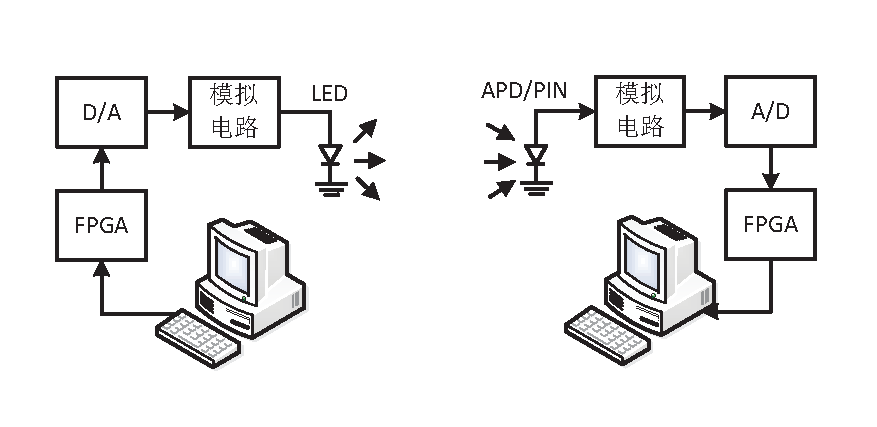
\includegraphics[width=0.8\textwidth]{figures/chapter-5/Hardware_Structure.eps}
\caption{可见光通信硬件平台示意图}
\label{fig:Hardware_Structure}
\end{figure}

首先信源比特通过以太网接口(UDP协议)按帧发送到用于基带处理的FPGA芯片(整个传输过程都是按帧进行的,并且用于同步和信道估计的ZC序列符号只在帧头处放置,整个帧中所有的OFDM符号都使用这个ZC序列估计出来的信道参数解调),接着在FPGA中完成扰码、信道编码、调制和IFFT等数字处理过程,然后将时域数字信号输入到数字模拟变换器(Digital to Analogue Converter,DAC)变成模拟信号,最后该模拟信号加上偏置电流之后去驱动LED灯,整个发射过程完成。接收端通过PD 接收LED光信号,并将光信号强弱的变化转换成电信号的大小,然后将此模拟电信号送入模拟/数字变换器(Analog to Digital Converter,ADC)中抽样量化为数字信号,再送到接收端基带处理FPGA进行解调、解码和校验等操作,最后输出接收到的帧到接收端计算机。
\subsection{硬件型号及参数简介}
本系统中用于基带处理的FPGA芯片选择美国Xilinx公司生产的Virtex-6,具体型号为XC6VSX315T,基于40 nm工艺,具有高性能、接口丰富等多方面优点。该芯片内部包含49,200个片逻辑单位,每个片逻辑单元中有4个查找表(Look Up Table,LUT)和8个触发器;内置1,344个DSP48数值计算块,每个数值计算块中包含一个$25\times 18$bit 乘法器、一个加法器和一个累加器;同时还有最大存储容量为25,244 kb的嵌入式存储RAM;并且支持千兆网卡\cite{FPGAIntroduciton}。这些资源为我们下面的基带逻辑处理及复杂的LDPC解码运算提供了硬件基础。

DAC选用美国TI公司生成的八通道高速数模转换芯片,型号为DAC3484,其输入数值信号位宽为16 bit,最高支持1 GSps的采样率;ADC芯片同样使用TI公司产品,型号为DAC9643,该芯片支持最高达250 MHz的采样速率,量化精度为14比特。

发射端模拟电路主要包括三部分,功率放大器、直流偏置模块和LED灯。功率放大器选用美国Mini-Circuits公司的ZHL-3A中功率放大器,其3 dB 带宽范围是0.4 MHz ~150 MHz,功率增益25 dB,最大输出功率为 30 dBm;采用的直流偏置模块ZFBT-6GW+同样是Mini-Circuits公司产品,其3 dB带宽范围为0.1 MHz~6 GHz,支持最大偏置电流0.5 A。发光二极管选用美国硅谷光擎(LED Engin)生产的多色混光型发光二极管LED——LZC-03MA07,其发光光谱图如图\ref{fig:LED_LZ4_relativeSputrcalPower}所示。

接收端模拟电路主要由滤光片、光电二极管即放大器。本系统为可见光多波段通信系统,不同的色光用不同的滤波片,分别是蓝光滤光片DTB435、绿光滤光片DTB530、红光滤光片HB610。光电转换模块选用雪崩型光电二极管(APD),具体型号为C5331-11,生产商为日本滨松公司(Hamamatsu),其3 dB通带为4 KHz~100 MHz,感光区直径1 mm。 接收端低噪声放大器选用美国TI公司生成的OPA847,其带宽增益积为3.9 GHz,输入噪声为$0.85 nV/\sqrt{Hz}$
\subsection{发射端基带处理}
\begin{figure}[htbp]
\centering
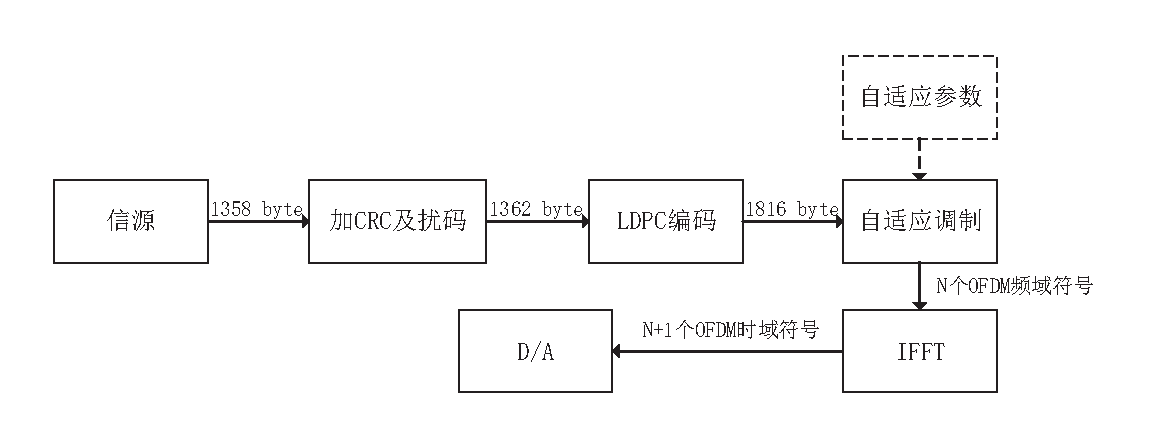
\includegraphics[width=0.9\textwidth]{figures/chapter-5/TransmitterSchematic.eps}
\caption{发射端基带处理原理框图}
\label{fig:TransmitterSchematic}
\end{figure}
发射端FPGA基带处理流程如图\ref{fig:TransmitterSchematic}所示,本演示系统信源帧长定为1358 byte (设置为该值主要是因为本系统主要以视频传输演示为主,而视频帧帧长就是1358 byte),为了系统设计简便起见,当通过以太网接口接到的帧不足1358 byte 时,会自动在后面补零再传输。

基带处理芯片接收到信源帧之后,第一步就是对其加循环冗余校验(Cyclic Redundancy Check,C RC),这里我们使用24 bit 的循环校验码,循环校验比特的生成模块其实就是一个由生成多项式决定的除法电路,输入数据就是被除数,而余数就是我们需要的校验比特,当然为了加快计算速度,本系统CRC使用8位并行计算方法,即不是想真的除法电路那样逐比特地输入,而是一次输入8 比特,整个运算速度提高了8倍。由于篇幅限制,在这里就不对CRC模块再进行过多的展开。得到24 bit(3 byte)校验位之后添加到原信源数据之后,又因为本系统使用的是输入为1362 byte 的低密度奇偶校验码(Low Density Parity Code,LDPC)作为信道编码,所以1358 byte数据帧加入3 byte 的校验码之后还要补零1 byte。为了防止过长的连0连1影响系统传输性能,所以还要把加了CRC及补零后的数据进行扰码再送入LDPC编码器。

信道编码是通过在发射数据中增加冗余以便在接收端可以进行信道解码纠错,本系统使用码率为3/4的LDPC码,输入数据长度为$1362\times 8$ bit,输出为14528 bit选择LDPC码的原因是其纠错性能佳,几乎适合所有信道,并且相对于Turbo码而言其解码器实现复杂度要低很多。这里使用的LDPC码的编码矩阵大小为$48\times 227$,所以输入数据位宽要为48 bit,而我们在CRC模块中输出数据位宽为8 bit,所以这里需要位宽变换,可以使用FPGA提供的RAM或先入先出队列(First In First Out,FIFO)数据结构来实现。编码之后的校验比特插在等间隔的插在信息数据中间,因为码率为3/4,每6字节信息数据后插入2个校验字节。

\begin{figure}[htbp]
\centering
\includegraphics[width=0.9\textwidth]{figures/chapter-5/TimeSchemeTrans.eps}
\caption{发射端基带处理时序图}
\label{fig:TimeSchemeTrans}
\end{figure}
经过编码的帧数据长度变为1816 byte,送入自适应调制模块,其功能是将信息比特分配到OFDM各个子载波上,并映射到星座图中的点,输出OFDM符号频域数据,这部分属于自适应设计的核心部分,将在下一节详细介绍。

经自适应模块调制后得到N个OFDM符号,N的值也调制的选择有关,假设根据自适应参数每个OFDM符号传输R比特,则有N=$\lceil 14528/\text{R} \rceil$,其中$\lceil \cdot \rceil$表示向上取整运算。为了提高传输速率,要保证所有的操作在一个OFDM帧周期内完成,所以要将将已调制符号交替存入两个RAM中,进行乒乓操作,即如果自适应模块再往其中RAM中写数据,则IFFT模块应该在另一个RAM中读数据去进行IFFT运算,到下一帧时这两个RAM的角色交换。IFFT模块可以使用Xilinx 公司提供的IP核实现,并且可以通过设置自动添加添加循环前缀,非常方便。得到OFDM时域符号之后,在每帧的头部再加上ZC导频序列之后输入到DAC芯片输出,整个发射过程的时序安排如图\ref{fig:TimeSchemeTrans}所示。
\subsection{接收端基带处理}
\begin{figure}[htbp]
\centering
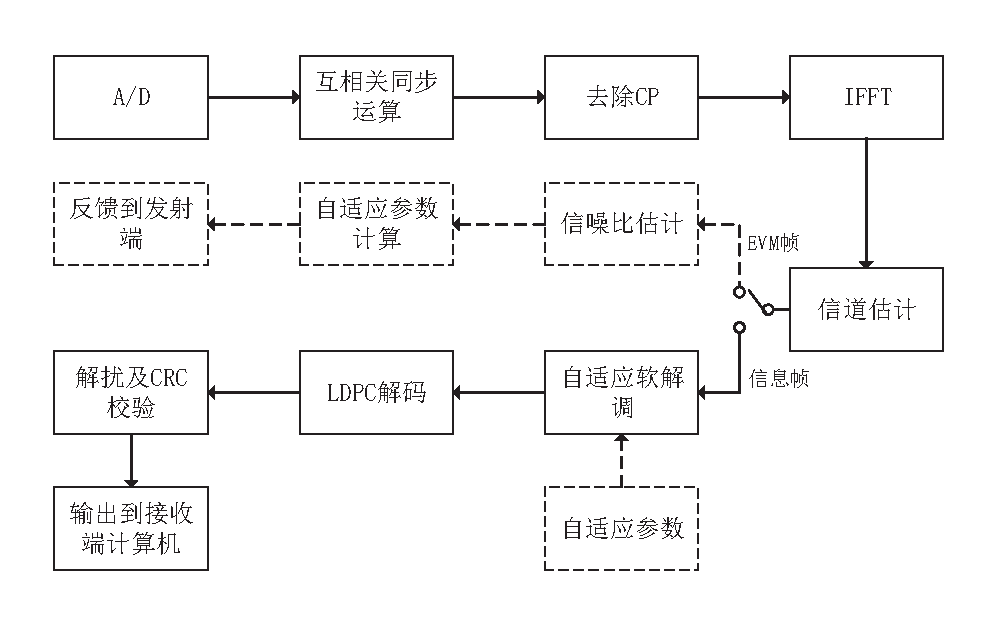
\includegraphics[width=0.9\textwidth]{figures/chapter-5/ReciverSchematic.eps}
\caption{接收端基带处理原理框图}
\label{fig:ReciverSchematic}
\end{figure}
接收端基带处理过程如图\ref{fig:ReciverSchematic}所示,模拟信号经过AD变化之后先与导频时域ZC 序列进行互相关同步运算,互相关结果的峰值所在位置就是导频的开始位置,在现实时为了避免找最大值这样复杂的运算,会通过另外一个模块估计接收信号的功率,从而得到一个互相关阀值,如果互相关结果大于这个阀值就可以认为是同步峰。使用这个特性就能把接收到的信号重新分成一个个OFDM符号,包含1个导频符号和N个信息符号。

因为要使用EVM方法进行信噪比估计,此时需要将用于EVM估计的前导序列放在信息符号发送,我们称这种帧为EVM帧。将这些时域OFDM符号去掉CP,再送入FFT模块,FFT模块输出频域OFDM符号,其中导频符号用于信道估计(使用LS算法),待得到信道估计之后,对信息符号进行单系数均衡,如果是数据帧则送入自适应软解调模块就行解调;如果是EVM帧怎送入信噪比估计模块估计SNR,之后再使用Improved-SBLA算法计算自适应参数,反馈到发射端,这部分也将在下一节展开。
\begin{figure}[htbp]
\centering
\includegraphics[width=0.9\textwidth]{figures/chapter-5/TimeSchemeRece.eps}
\caption{接收端基带处理时序图}
\label{fig:TransmitterSchematic}
\end{figure}

软解调得到的软件被送入LDPC码解码模块进行解码,软解调的输出位宽因调制阶数不同不同,如使用4QAM调制的子载波软解调输出位宽为16($8\times 2$)bit、16QAM为32 ($8\times 4$)bit、64QAM为48($8\times 6$)bit、256QAM对应为64($8\times 8$)bit,而解码器的输入位宽为$256=8\times 32$ bit,所以这里也存在数据位宽变换的问题,可以先将各阶调制得到的软量存在各自的RAM中,然后统一以64 bit位宽读出到一个FIFO中,再以256 bit位宽读出送入LDPC解码器解码。如接收端基带处理时序图\ref{fig:TransmitterSchematic}所示,解码过程所需要的时间也迭代次数成正比,具体为迭代次数加1再乘以227,本系统设置迭代次数为20,故整个解码过程为4767 clk。 解码器输出位宽为48 bit,经位宽变换为8 bit 之后送入CRC模块进行校验,以统计误帧率,这是系统QoS一个重要的指标。如果通过CRC校验帧正确,则通过以太网接口送入接收端计算机,否则丢弃该帧。


\section{自适应模块方案设计}
上节从硬件参数到基带设计对整个硬件平台进行了简略的介绍,我们已经对整个系统有了一定的认识。在原来的系统上实现自适应传输功能只需就行几个模块的改造,而发射端编码器及之前、接收端译码器及之后等部分都不要变。下面详细介绍这几个涉及到自适应传输的模块。
\subsection{自适应调制模块}
\begin{figure}[htbp]
\centering
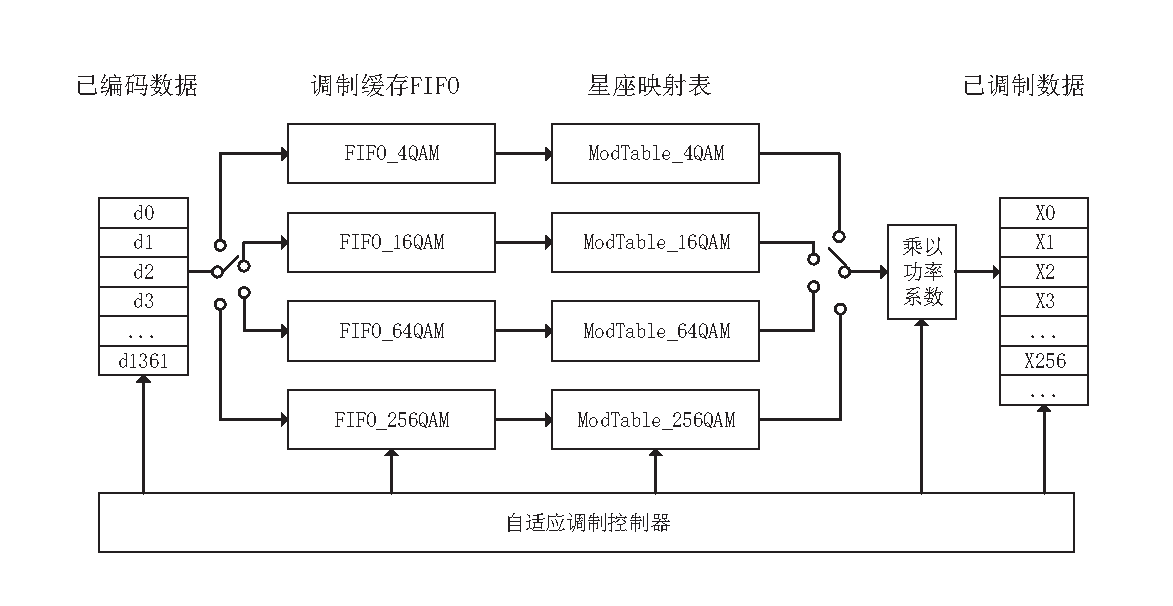
\includegraphics[width=0.9\textwidth]{figures/chapter-5/AdaptiveModulation.eps}
\caption{自适应调制模块示意图}
\label{fig:AdaptiveModulation}
\end{figure}
发射端的自适应调制模块设计如图\ref{fig:AdaptiveModulation}所示,已完成信道编码的数据放在一个位宽为8 bit的RAM中,现在要将这些数据分配到各个子载波上,本系统设计中我们的调制方式限定为4QAM、16QAM、64QAM和256QAM,而每种不同的调制每个符号能够携带的信息比特数也不同,每个M-QAM携带的比特数为$\log_2(M)$。因此先要把已编码的数据根据比特分配表放到不同的FIFO中去,因为FIFO的性质是FIFO的数据位宽要是输入输出的位宽的倍数,所以用于缓存FIFO的位宽及输入输出位宽如下表所示:
\begin{table}[ht]
    \caption{调制器FIFO参数设置}
    \label{tab:Signle Color Channel Estimation Paramters}
    \centering
    \begin{tabular}{llll}
        \toprule
        FIFO                & 数据位宽  &输入位宽  &输出位宽\\
        \midrule
		FIFO\_4QAM			& 8 bit		&8 bit    & 2 bit  \\
		FIFO\_16QAM			& 8 bit       &8 bit    & 4 bit  \\
		FIFO\_64QAM          & 24 bit       &24 bit    & 6 bit   \\
		FIFO\_64QAM			& 8 bit         &8 bit    & 8 bit  \\
        \bottomrule
    \end{tabular}
\end{table}
所以对于64QAM调制,缓存时需要先拼成24 bit输入,在以6 bit位宽读出。

数据缓存之后,使用查表法进行星座映射。具体是先把各阶QAM调制的已归一化星座点存到不同的ROM中,实部和虚部都按14 bit量化,然后按照各个子载波上的调制阶数,依次从各个FIFO中读出数据,并以此数据为地址,去读该调制下的星座图ROM,输出的数据就是归一化过的星座点,最后再根据功率分配表,乘上功率系数之后存到RAM缓存,同时要注意与之前固定调制不同,这里考虑的功率分配的因素,所以为了接收端简化起见,要在导频ZC序列上各个子载波也要乘以功率系数,这样接收端在解调的时候就不要再专门除以功率系数,会在单系数均衡中处理掉。整个自适应调制器由一个专门的控制器模块来进行时序控制和状态转换。

\subsection{信噪比估计与自适应参数计算}
\begin{figure}[htbp]
\centering
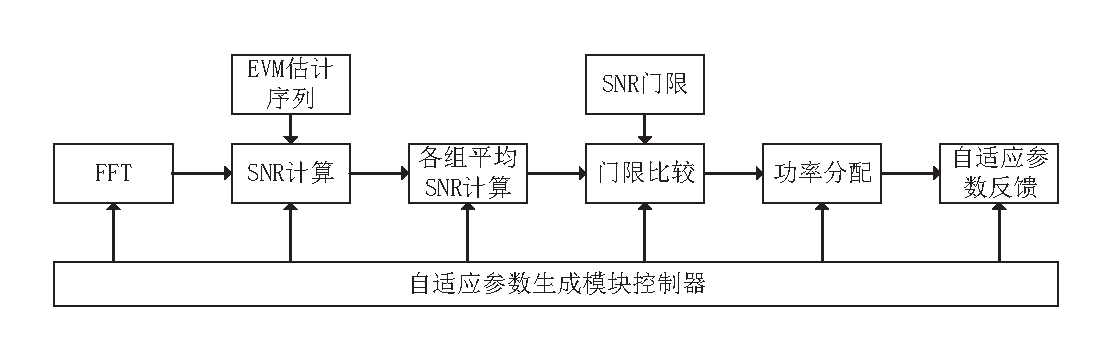
\includegraphics[width=0.9\textwidth]{figures/chapter-5/AdaptiveParameterGenerator.eps}
\caption{自适应参数生成模块示意图}
\label{fig:AdaptiveParameterGenerator}
\end{figure}
信噪比估计及自适应参数计算方案设计如图\ref{fig:AdaptiveParameterGenerator}所示,之前也提过,系统要传输专门的EVM序列来进行SNR估计,这样的帧成为EVM 帧,可以隔固定的时间发送一次,所以处理EVM帧其实就是求当前信道下的自适应参数。

EVM序列频域符号在接收端也是已知的,所以得到已经均衡过的时域符号之后,可以根据公式求得各个子载波上的SNR和噪声方差,每个OFDM符号都能得到一组SNR和噪声方差,可以通过几组值相加求平均的方法来提高估计精度。得到各个子载波上的SNR之后,根据设置的子载波总数和组数,求得每组子载波的平均SNR,然后利用Improved-SBLA 算法来进行比特和功率分配,为了简便起见,保证系统的鲁棒性,我们设置目标BER为$10^{-2}$,同时只按原算法进行初始分配,而不设置目标速率,这样就少了算法后来的循环累加或类减过程。在门限比较时,可以从高门限到低门限比较,当遇到SNR大于某个门限时,就取其对应的调制阶数。得到各个子载波组上分配的比特之后,使用公式求得各个子载波组的第一个子载波和最后一个子载波的功率。将此比特分配和功率分配按照一定的数据格式发送给发射端。
\subsection{自适应软解调模块}
\begin{figure}[htbp]
\centering
\includegraphics[width=0.9\textwidth]{figures/chapter-5/AdaptiveDemodulation.eps}
\caption{自适应软解调模块示意图}
\label{fig:AdaptiveDemodulation}
\end{figure}
当传输的是数据帧时,自适应软解调按图\ref{fig:AdaptiveDemodulation}所示方案进行软解调,其基本思路是查表法,并且只使用256QAM调制一张表,其他的三种低阶调制通过一些数据变换来时候这张表,按照软量计算理论,实部和虚部分开进行软量计算,并且使用的方法是一样的。下面来介绍具体过程。

经过了单系数均衡后的各个子载波上的频域符号先要进行幅度调制,即乘以其对应的调制阶数的归一化因子,恢复各个调制符号在原始星座图上的幅度,并且要根据调制阶数进行相应的饱和处理,将其限定在对应星座图的范围内,如256-QAM限定在(-16,16)的范围内,64-QAM限定在(-8,8)范围内。然后采用坐标平移的方法让低阶调制能够使用256QAM的软量表,需要对其坐标点搬移到最高阶调制星座图上的合适位置。首先读取当前子载波所用的调制阶数以进行判断,从最低的4QAM移动到16QAM 坐标值减2,16QAM移动到64QAM坐标值减4,以此类推,即$2^k$-QAM向高阶移一阶坐标值减$2^k$/2。因此,对于本设计中各种调制都要移动到256QAM上,256QAM 本身不用移动,64QAM 要减去8,16QAM减去12,4QAM减去14。这样处理完了之后的实部和虚部数据就可以去查软量表了。因为对应的软量是256QAM的,并且软量是按8 bit 量化的,所以从软量表输出的是 32($4\times 8$)bit软量,而低阶调制只是取其中的一部分,如4QAM实部和虚部各传输1 bit,所以取软量表输出最后的8 bit,依次类推就能得到所有的比特软量了。从前所述不难看出,各个OFDM子载波因为调制阶数的不同,所以生成比特软量的速率也不同,所以要把得到的软量按顺序缓存下来,再送入LDPC译码器。

\section{系统展示}
本课题设计的硬件平台如图\ref{fig:Demo}所示,左边的三台计算机用于产生发射信源,T\_Red、T\_Blue和T\_Green发出的数据分别通过多色LED 的红光、蓝光和绿光三个通道发送到接收端;右边三台计算机R\_red、R\_Blue和R\_Green接收响应色光的数据并显示。

\begin{figure}[htbp]
\centering
\includegraphics[width=0.9\textwidth]{figures/chapter-5/Demo.jpg}
\caption{硬件平台展示}
\label{fig:Demo}
\end{figure}




\section{本章小结}
本章在前面几章讲解可见光通信原理及其自适应传输理论的基础上,介绍了本课题对应的硬件平台。首先对整个硬件平台进行了概述,包括各种器件的参数及其选择依据,并且简述了发射端和接收端的基带处理处理过程;然后重点描述了基带处理中与自适应技术密切相关的调制器、自适应参数生成、软解调三个模块;最后展示了整个硬件平台实物图。
%    \chapter{全文总结与展望}
本课题主要讨论了可见光多波段通信领域的自适应传输技术,包括可见光通信的基本原理、信道估计及自适应比特功率分配算法等,最后给出了系统硬件设计方案,下面对全文进行简要的总结并分析该领域之后的研究方向。
\section{论文工作总结}
第一章是绪论。主要介绍了可见光通信的研究背景,包括其应用场景及与传统通信方式相比的优势,同时也对可见光通信在国内外的发展历程进行了概述。

第二章首先可见光通信的基本原理,包括系统模型、信道特征及光电元器件等,本文联系实际情况将可见光通信信道建模为线性信道,然后介绍了电光转换器件LED,详细说明了荧光激发型LED和多色混合型LED的工作原理和特性,还介绍PIN 和APD两类光电转换器件及接收端使用的滤光片。理解这些光电元器件的原理与作用有益于理解整个可见光通信系统。由于OFDM调制技术非常适应光低通信道,在可见光通信中也得到了广泛的使用,所以本章也介绍了光OFDM技术,主要说明了DCO-OFDM和ACO-OFDM的工作原理及区别,在此基础上提出了一种改善ACO-OFDM 系统PAPR 性能的RoC-ACO-OFDM方案,并且在理论和数值仿真的角度论证了该方案的有效性。

第三章主要分析了OFDM信道估计方法的基本原理及其在可见光通信中的应用,首先探讨了OFDM信道估计的常用方法,重点放在基于导频的方法中,系统研究了基于最小二乘法的LS信号估计方法、基于最小均方误差的MMSE方法及其基于MMSE两个改进方法LMMSE和SVD分解方法;然后结合可见光通信系统设计的实例,使用ZC序列作为导频,通过仿真的方法比较了上述方法在可见光信道下的性能,发现虽然LS 信道估计方法在本系统工作点(SNR=25 dB)附近性能稍逊于LMMSE及SVD算法,但是其实现要简便得多,所以在本课题硬件设计中将采用LS进行信道估计;最后讨论了OFDM系统中信噪比的估计方法,分析了基于导频的估计方法和EVM方法,得出了EVM方法虽然需要额外的开销,但是其估计值更加吻合实际系统,推荐在可见光自适应传输系统中使用该方法。

第四章主要介绍了OFDM系统的比特和功率分配算法,研究其在可见光通信中的应用,选出了适合可见光通信的SBLA分配算法,并且在此算法的基础上进行了改进。首先阐述了自适应传输的理论基础—香农信息论和注水定理;然后说明了自适应传输的三种优化准则,即固定目标误比特率和发射功率的最大速率准则(RA)、固定目标误比特率和速率的最小发射功率准则(MA)及固定发射功率和速率的最小误比特率准则(BA),再次基础上介绍了OFDM自适应传输领域三个最经典的算法,分别是在RA和MA准则下最优的Hughes-Hartogs算法、BA准则下Chow算法和Fischer算法,详细说明了这些算法的推导和实现步骤,并且通过仿真比较了它们的性能差异,发现在可见光通信信道下它们在BA准则下BER性能相差不大;最后分析了适合子载波SNR相关性较大的SBLA算法,因此可见光信道本身就是低通的,天然合适SBLA算法的应用,并且进一步利用可见光通信信道特征,提出了适应线性插值来进行功率分配的Improved-SBLA算法,通过仿真发现改进的算法在减少了反馈量就运算复杂度的基础上,BER性能与SBLA相当,说明改进算法是合理可行的。

第五章在前面几章讲解可见光通信原理及其自适应传输理论的基础上,介绍了本课题对应的硬件平台。首先对整个硬件平台进行了概述,包括各种器件的参数及其选择依据,并且简述了发射端和接收端的基带处理处理过程;然后重点描述了基带处理中与自适应技术密切相关的调制器、自适应参数生成、软解调三个模块;最后展示了整个硬件平台实物图。

第六章对全文进行简要的总结并分析该领域之后的研究方向。
\section{展望}
要进行自适应传输,首要条件就是实现双向通信,而目前室内可见光通信的反向链路还没有明确的方案,这个是可见光通信要亟待解决的问题,所以我认为这个领域将引起越来越多研究人员的注意。

另外现在很多研究人员在尝试通过不同的途径来提高可见光通信的传输速率,但针对系统可靠性的研究还不多,特别是在没有直达径下的通信场景,这方面的研究在以后可能也会成为热点。
\end{Main}
% 结束正文

% 参考文献
\bibliography{Reference}

% 附录
%% !Mode:: "TeX:UTF-8"
% 附录

\begin{Appendix}
	\chapter{第一个附录}
	\chapter{第二个附录}
\end{Appendix}
%%%%%%%%%%%%%%%%%%%%论文结尾%%%%%%%%%%%%%%%%%%%%%%%
%\newpage
%\printindex % 索引
%
%% !Mode:: "TeX:UTF-8"

\begin{Resume}
%\fontsize{12pt}{14pt}\selectfont
    \begin{itemize}
        \item 期刊论文
            \begin{itemize}
                \item 第二作者, ``ACO-OFDM-Specified Recoverable Upper Clipping With Efficient Detection for Optical Wireless Communications''.  Photonics Journal, IEEE, 2014, 6(5): 1-17.
                %\item 第一作者, 第二作者, 第三作者, ``Incremental scheduling scheme for indoor visible light communication'', Electronics Letters, Jan. 2015, Accepted.
            \end{itemize}
        \item 专利
            \begin{itemize}
                \item 第二发明人, `` 一种采用削波搬移的低峰均比无线光传输方法'', 申请号:201410206887.X, 2014年5 月.
                %\item ``一种分布式组网光通信系统的灯组协同调度方法'', 申请号:201410191671.0, 2014年6月.
            \end{itemize}
            \begin{itemize}
                \item 第二发明人, `` 一种多色LED可见光通信自适应传输方法'', 申请号:201510019678.9, 2015 年 1月.
                %\item ``一种分布式组网光通信系统的灯组协同调度方法'', 申请号:201410191671.0, 2014年6月.
            \end{itemize}
    \end{itemize}
\end{Resume}
 % 个人简介
%
%\include{Acknowledgement} % 致谢
%%%%%%%%%%%%%%%%%%%% End of 论文结尾%%%%%%%%%%%%%%%

\end{document}
